% Options for packages loaded elsewhere
% Options for packages loaded elsewhere
\PassOptionsToPackage{unicode}{hyperref}
\PassOptionsToPackage{hyphens}{url}
\PassOptionsToPackage{dvipsnames,svgnames,x11names}{xcolor}
%
\documentclass[
  letterpaper,
  DIV=11,
  numbers=noendperiod]{scrartcl}
\usepackage{xcolor}
\usepackage{amsmath,amssymb}
\setcounter{secnumdepth}{5}
\usepackage{iftex}
\ifPDFTeX
  \usepackage[T1]{fontenc}
  \usepackage[utf8]{inputenc}
  \usepackage{textcomp} % provide euro and other symbols
\else % if luatex or xetex
  \usepackage{unicode-math} % this also loads fontspec
  \defaultfontfeatures{Scale=MatchLowercase}
  \defaultfontfeatures[\rmfamily]{Ligatures=TeX,Scale=1}
\fi
\usepackage{lmodern}
\ifPDFTeX\else
  % xetex/luatex font selection
\fi
% Use upquote if available, for straight quotes in verbatim environments
\IfFileExists{upquote.sty}{\usepackage{upquote}}{}
\IfFileExists{microtype.sty}{% use microtype if available
  \usepackage[]{microtype}
  \UseMicrotypeSet[protrusion]{basicmath} % disable protrusion for tt fonts
}{}
\makeatletter
\@ifundefined{KOMAClassName}{% if non-KOMA class
  \IfFileExists{parskip.sty}{%
    \usepackage{parskip}
  }{% else
    \setlength{\parindent}{0pt}
    \setlength{\parskip}{6pt plus 2pt minus 1pt}}
}{% if KOMA class
  \KOMAoptions{parskip=half}}
\makeatother
% Make \paragraph and \subparagraph free-standing
\makeatletter
\ifx\paragraph\undefined\else
  \let\oldparagraph\paragraph
  \renewcommand{\paragraph}{
    \@ifstar
      \xxxParagraphStar
      \xxxParagraphNoStar
  }
  \newcommand{\xxxParagraphStar}[1]{\oldparagraph*{#1}\mbox{}}
  \newcommand{\xxxParagraphNoStar}[1]{\oldparagraph{#1}\mbox{}}
\fi
\ifx\subparagraph\undefined\else
  \let\oldsubparagraph\subparagraph
  \renewcommand{\subparagraph}{
    \@ifstar
      \xxxSubParagraphStar
      \xxxSubParagraphNoStar
  }
  \newcommand{\xxxSubParagraphStar}[1]{\oldsubparagraph*{#1}\mbox{}}
  \newcommand{\xxxSubParagraphNoStar}[1]{\oldsubparagraph{#1}\mbox{}}
\fi
\makeatother

\usepackage{color}
\usepackage{fancyvrb}
\newcommand{\VerbBar}{|}
\newcommand{\VERB}{\Verb[commandchars=\\\{\}]}
\DefineVerbatimEnvironment{Highlighting}{Verbatim}{commandchars=\\\{\}}
% Add ',fontsize=\small' for more characters per line
\usepackage{framed}
\definecolor{shadecolor}{RGB}{241,243,245}
\newenvironment{Shaded}{\begin{snugshade}}{\end{snugshade}}
\newcommand{\AlertTok}[1]{\textcolor[rgb]{0.68,0.00,0.00}{#1}}
\newcommand{\AnnotationTok}[1]{\textcolor[rgb]{0.37,0.37,0.37}{#1}}
\newcommand{\AttributeTok}[1]{\textcolor[rgb]{0.40,0.45,0.13}{#1}}
\newcommand{\BaseNTok}[1]{\textcolor[rgb]{0.68,0.00,0.00}{#1}}
\newcommand{\BuiltInTok}[1]{\textcolor[rgb]{0.00,0.23,0.31}{#1}}
\newcommand{\CharTok}[1]{\textcolor[rgb]{0.13,0.47,0.30}{#1}}
\newcommand{\CommentTok}[1]{\textcolor[rgb]{0.37,0.37,0.37}{#1}}
\newcommand{\CommentVarTok}[1]{\textcolor[rgb]{0.37,0.37,0.37}{\textit{#1}}}
\newcommand{\ConstantTok}[1]{\textcolor[rgb]{0.56,0.35,0.01}{#1}}
\newcommand{\ControlFlowTok}[1]{\textcolor[rgb]{0.00,0.23,0.31}{\textbf{#1}}}
\newcommand{\DataTypeTok}[1]{\textcolor[rgb]{0.68,0.00,0.00}{#1}}
\newcommand{\DecValTok}[1]{\textcolor[rgb]{0.68,0.00,0.00}{#1}}
\newcommand{\DocumentationTok}[1]{\textcolor[rgb]{0.37,0.37,0.37}{\textit{#1}}}
\newcommand{\ErrorTok}[1]{\textcolor[rgb]{0.68,0.00,0.00}{#1}}
\newcommand{\ExtensionTok}[1]{\textcolor[rgb]{0.00,0.23,0.31}{#1}}
\newcommand{\FloatTok}[1]{\textcolor[rgb]{0.68,0.00,0.00}{#1}}
\newcommand{\FunctionTok}[1]{\textcolor[rgb]{0.28,0.35,0.67}{#1}}
\newcommand{\ImportTok}[1]{\textcolor[rgb]{0.00,0.46,0.62}{#1}}
\newcommand{\InformationTok}[1]{\textcolor[rgb]{0.37,0.37,0.37}{#1}}
\newcommand{\KeywordTok}[1]{\textcolor[rgb]{0.00,0.23,0.31}{\textbf{#1}}}
\newcommand{\NormalTok}[1]{\textcolor[rgb]{0.00,0.23,0.31}{#1}}
\newcommand{\OperatorTok}[1]{\textcolor[rgb]{0.37,0.37,0.37}{#1}}
\newcommand{\OtherTok}[1]{\textcolor[rgb]{0.00,0.23,0.31}{#1}}
\newcommand{\PreprocessorTok}[1]{\textcolor[rgb]{0.68,0.00,0.00}{#1}}
\newcommand{\RegionMarkerTok}[1]{\textcolor[rgb]{0.00,0.23,0.31}{#1}}
\newcommand{\SpecialCharTok}[1]{\textcolor[rgb]{0.37,0.37,0.37}{#1}}
\newcommand{\SpecialStringTok}[1]{\textcolor[rgb]{0.13,0.47,0.30}{#1}}
\newcommand{\StringTok}[1]{\textcolor[rgb]{0.13,0.47,0.30}{#1}}
\newcommand{\VariableTok}[1]{\textcolor[rgb]{0.07,0.07,0.07}{#1}}
\newcommand{\VerbatimStringTok}[1]{\textcolor[rgb]{0.13,0.47,0.30}{#1}}
\newcommand{\WarningTok}[1]{\textcolor[rgb]{0.37,0.37,0.37}{\textit{#1}}}

\usepackage{longtable,booktabs,array}
\usepackage{calc} % for calculating minipage widths
% Correct order of tables after \paragraph or \subparagraph
\usepackage{etoolbox}
\makeatletter
\patchcmd\longtable{\par}{\if@noskipsec\mbox{}\fi\par}{}{}
\makeatother
% Allow footnotes in longtable head/foot
\IfFileExists{footnotehyper.sty}{\usepackage{footnotehyper}}{\usepackage{footnote}}
\makesavenoteenv{longtable}
\usepackage{graphicx}
\makeatletter
\newsavebox\pandoc@box
\newcommand*\pandocbounded[1]{% scales image to fit in text height/width
  \sbox\pandoc@box{#1}%
  \Gscale@div\@tempa{\textheight}{\dimexpr\ht\pandoc@box+\dp\pandoc@box\relax}%
  \Gscale@div\@tempb{\linewidth}{\wd\pandoc@box}%
  \ifdim\@tempb\p@<\@tempa\p@\let\@tempa\@tempb\fi% select the smaller of both
  \ifdim\@tempa\p@<\p@\scalebox{\@tempa}{\usebox\pandoc@box}%
  \else\usebox{\pandoc@box}%
  \fi%
}
% Set default figure placement to htbp
\def\fps@figure{htbp}
\makeatother


% definitions for citeproc citations
\NewDocumentCommand\citeproctext{}{}
\NewDocumentCommand\citeproc{mm}{%
  \begingroup\def\citeproctext{#2}\cite{#1}\endgroup}
\makeatletter
 % allow citations to break across lines
 \let\@cite@ofmt\@firstofone
 % avoid brackets around text for \cite:
 \def\@biblabel#1{}
 \def\@cite#1#2{{#1\if@tempswa , #2\fi}}
\makeatother
\newlength{\cslhangindent}
\setlength{\cslhangindent}{1.5em}
\newlength{\csllabelwidth}
\setlength{\csllabelwidth}{3em}
\newenvironment{CSLReferences}[2] % #1 hanging-indent, #2 entry-spacing
 {\begin{list}{}{%
  \setlength{\itemindent}{0pt}
  \setlength{\leftmargin}{0pt}
  \setlength{\parsep}{0pt}
  % turn on hanging indent if param 1 is 1
  \ifodd #1
   \setlength{\leftmargin}{\cslhangindent}
   \setlength{\itemindent}{-1\cslhangindent}
  \fi
  % set entry spacing
  \setlength{\itemsep}{#2\baselineskip}}}
 {\end{list}}
\usepackage{calc}
\newcommand{\CSLBlock}[1]{\hfill\break\parbox[t]{\linewidth}{\strut\ignorespaces#1\strut}}
\newcommand{\CSLLeftMargin}[1]{\parbox[t]{\csllabelwidth}{\strut#1\strut}}
\newcommand{\CSLRightInline}[1]{\parbox[t]{\linewidth - \csllabelwidth}{\strut#1\strut}}
\newcommand{\CSLIndent}[1]{\hspace{\cslhangindent}#1}



\setlength{\emergencystretch}{3em} % prevent overfull lines

\providecommand{\tightlist}{%
  \setlength{\itemsep}{0pt}\setlength{\parskip}{0pt}}



 


\usepackage{newunicodechar}
\newunicodechar{ʻ}{`}
\renewcommand{\thefigure}{S\arabic{figure}}
\renewcommand{\thesection}{S\arabic{section}}
\KOMAoption{captions}{tableheading}
\makeatletter
\@ifpackageloaded{caption}{}{\usepackage{caption}}
\AtBeginDocument{%
\ifdefined\contentsname
  \renewcommand*\contentsname{Table of contents}
\else
  \newcommand\contentsname{Table of contents}
\fi
\ifdefined\listfigurename
  \renewcommand*\listfigurename{List of Figures}
\else
  \newcommand\listfigurename{List of Figures}
\fi
\ifdefined\listtablename
  \renewcommand*\listtablename{List of Tables}
\else
  \newcommand\listtablename{List of Tables}
\fi
\ifdefined\figurename
  \renewcommand*\figurename{Supplementary Figure}
\else
  \newcommand\figurename{Supplementary Figure}
\fi
\ifdefined\tablename
  \renewcommand*\tablename{Table}
\else
  \newcommand\tablename{Table}
\fi
}
\@ifpackageloaded{float}{}{\usepackage{float}}
\floatstyle{ruled}
\@ifundefined{c@chapter}{\newfloat{codelisting}{h}{lop}}{\newfloat{codelisting}{h}{lop}[chapter]}
\floatname{codelisting}{Listing}
\newcommand*\listoflistings{\listof{codelisting}{List of Listings}}
\makeatother
\makeatletter
\makeatother
\makeatletter
\@ifpackageloaded{caption}{}{\usepackage{caption}}
\@ifpackageloaded{subcaption}{}{\usepackage{subcaption}}
\makeatother
\usepackage{bookmark}
\IfFileExists{xurl.sty}{\usepackage{xurl}}{} % add URL line breaks if available
\urlstyle{same}
\hypersetup{
  pdftitle={Supplement to ``Eco-evolutionary deviations from steady state across the Hawaiian chronosequence from a maximum entropy perspective''},
  colorlinks=true,
  linkcolor={blue},
  filecolor={Maroon},
  citecolor={Blue},
  urlcolor={Blue},
  pdfcreator={LaTeX via pandoc}}


\title{Supplement to ``Eco-evolutionary deviations from steady state
across the Hawaiian chronosequence from a maximum entropy perspective''}
\author{}
\date{}
\begin{document}
\maketitle


This supplement walks through the steps of recreating the entire
analysis presented in the main text. It also provides further analysis
in support of and to contextualize results in the main text.

\section{Computing setup}\label{computing-setup}

Analyses are supported by a custom R package \emph{HawaiiArthMETE}
(\textbf{foo?}) which can be installed from github.

\begin{Shaded}
\begin{Highlighting}[]
\NormalTok{devtools}\SpecialCharTok{::}\FunctionTok{install\_github}\NormalTok{(}\StringTok{"ecoevomatics/HawaiiArthMETE"}\NormalTok{)}
\end{Highlighting}
\end{Shaded}

The quarto (Allaire \emph{et al.} 2025) document used to generate this
supplement can be found with the R command
\texttt{system.file("ms/hawaii-arth-mete-supp.qmd",\ package\ =\ "HawaiiArthMETE")}.

The following R computing environment is used for all analyses:

\begin{Shaded}
\begin{Highlighting}[]
\FunctionTok{library}\NormalTok{(meteR)}
\FunctionTok{library}\NormalTok{(ggplot2)}
\FunctionTok{library}\NormalTok{(ggh4x)}
\FunctionTok{library}\NormalTok{(dplyr)}
\end{Highlighting}
\end{Shaded}

\begin{verbatim}

Attaching package: 'dplyr'
\end{verbatim}

\begin{verbatim}
The following objects are masked from 'package:stats':

    filter, lag
\end{verbatim}

\begin{verbatim}
The following objects are masked from 'package:base':

    intersect, setdiff, setequal, union
\end{verbatim}

\begin{Shaded}
\begin{Highlighting}[]
\FunctionTok{library}\NormalTok{(tidyr)}
\FunctionTok{library}\NormalTok{(metafor)}
\end{Highlighting}
\end{Shaded}

\begin{verbatim}
Loading required package: Matrix
\end{verbatim}

\begin{verbatim}

Attaching package: 'Matrix'
\end{verbatim}

\begin{verbatim}
The following objects are masked from 'package:tidyr':

    expand, pack, unpack
\end{verbatim}

\begin{verbatim}
Loading required package: metadat
\end{verbatim}

\begin{verbatim}
Loading required package: numDeriv
\end{verbatim}

\begin{verbatim}

Loading the 'metafor' package (version 5.0-1). For an
introduction to the package please type: help(metafor)
\end{verbatim}

\begin{Shaded}
\begin{Highlighting}[]
\FunctionTok{library}\NormalTok{(HawaiiArthMETE)}
\end{Highlighting}
\end{Shaded}

\begin{verbatim}

Attaching package: 'HawaiiArthMETE'
\end{verbatim}

\begin{verbatim}
The following object is masked from 'package:meteR':

    arth
\end{verbatim}

\begin{Shaded}
\begin{Highlighting}[]
\NormalTok{knitr}\SpecialCharTok{::}\NormalTok{opts\_chunk}\SpecialCharTok{$}\FunctionTok{set}\NormalTok{(}
    \CommentTok{\# default figure dims}
    \AttributeTok{fig.width =} \FloatTok{5.5}\NormalTok{, }\AttributeTok{fig.height =} \DecValTok{4}\NormalTok{, }
    \CommentTok{\# caching is default for all subsequent chunks}
    \AttributeTok{cache =} \ConstantTok{TRUE}
\NormalTok{)}

\CommentTok{\# load data }
\FunctionTok{data}\NormalTok{(arth)}

\FunctionTok{sessionInfo}\NormalTok{() }\SpecialCharTok{|\textgreater{}} 
    \FunctionTok{print}\NormalTok{(}\AttributeTok{locale =} \ConstantTok{FALSE}\NormalTok{)}
\end{Highlighting}
\end{Shaded}

\begin{verbatim}
R version 4.5.2 (2025-10-31)
Platform: aarch64-apple-darwin20
Running under: macOS Sequoia 15.0.1

Matrix products: default
BLAS:   /System/Library/Frameworks/Accelerate.framework/Versions/A/Frameworks/vecLib.framework/Versions/A/libBLAS.dylib 
LAPACK: /Library/Frameworks/R.framework/Versions/4.5-arm64/Resources/lib/libRlapack.dylib;  LAPACK version 3.12.1

attached base packages:
[1] stats     graphics  grDevices utils     datasets  methods   base     

other attached packages:
 [1] HawaiiArthMETE_0.1.0 metafor_5.0-1        numDeriv_2016.8-1.1 
 [4] metadat_1.6-0        Matrix_1.7-4         tidyr_1.3.1         
 [7] dplyr_1.2.1          ggh4x_0.3.1          ggplot2_4.0.1       
[10] meteR_1.2           

loaded via a namespace (and not attached):
 [1] gtable_0.3.6       jsonlite_2.0.0     compiler_4.5.2     tidyselect_1.2.1  
 [5] scales_1.4.0       yaml_2.3.10        fastmap_1.2.0      lattice_0.22-7    
 [9] R6_2.6.1           generics_0.1.4     knitr_1.50         tibble_3.3.0      
[13] pillar_1.11.0      RColorBrewer_1.1-3 rlang_1.2.0        mathjaxr_2.0-0    
[17] xfun_0.52          S7_0.2.1           cli_3.6.5          withr_3.0.2       
[21] magrittr_2.0.4     digest_0.6.39      grid_4.5.2         rstudioapi_0.17.1 
[25] nlme_3.1-168       lifecycle_1.0.5    vctrs_0.7.3        evaluate_1.0.4    
[29] glue_1.8.0         farver_2.1.2       rmarkdown_2.29     purrr_1.1.0       
[33] tools_4.5.2        pkgconfig_2.0.3    htmltools_0.5.8.1 
\end{verbatim}

\section{METE calculations}\label{mete-calculations}

Comparison of the observed data to predictions from the Maximum Entropy
Theory of Ecology (METE) is performed with package \emph{meteR}
(\textbf{rominger-merow2016?}). The following code records information
about each sample (name, flow age, proportion non-native presence) as
well as several metrics of deviation between theory and observation:

\begin{itemize}
\tightlist
\item
  a \(z^2\) value measuring a normalized difference in likelihoods
  between observed data and theoretical expectation
\item
  differences in proportion of rarity (number of singletons or
  normalized metabolic rate \(\leq 2\)) observed and expected
\item
  differences in proportion of dominance (sum of top three most abundant
  species or sum of top three highest normalized metabolic rates)
  observed and expected
\end{itemize}

All metrics are calculated for both the species abundance distribution
(SAD) and individual metabolic rate (or power) distribution (IPD).

\begin{Shaded}
\begin{Highlighting}[]
\NormalTok{arth\_mete }\OtherTok{\textless{}{-}} \FunctionTok{split}\NormalTok{(arth, arth[, }\FunctionTok{c}\NormalTok{(}\StringTok{"site"}\NormalTok{, }\StringTok{"tree"}\NormalTok{)], }\AttributeTok{drop =} \ConstantTok{TRUE}\NormalTok{) }\SpecialCharTok{|\textgreater{}} 
    \FunctionTok{lapply}\NormalTok{(}\ControlFlowTok{function}\NormalTok{(x) \{}
        \CommentTok{\# the esf for this grouping}
\NormalTok{        esf }\OtherTok{\textless{}{-}} \FunctionTok{meteESF}\NormalTok{(}\AttributeTok{spp =}\NormalTok{ x}\SpecialCharTok{$}\NormalTok{species\_code, }
                       \AttributeTok{abund =}\NormalTok{ x}\SpecialCharTok{$}\NormalTok{abundance, }
                       \AttributeTok{power =}\NormalTok{ x}\SpecialCharTok{$}\NormalTok{metabolic\_rate)}
        
        \CommentTok{\# sad and ipd}
\NormalTok{        s }\OtherTok{\textless{}{-}} \FunctionTok{sad}\NormalTok{(esf)}
\NormalTok{        p }\OtherTok{\textless{}{-}} \FunctionTok{ipd}\NormalTok{(esf)}
        
        \FunctionTok{data.frame}\NormalTok{(}
            \CommentTok{\# sample info}
            \AttributeTok{site =}\NormalTok{ x}\SpecialCharTok{$}\NormalTok{site[}\DecValTok{1}\NormalTok{],}
            \AttributeTok{site\_name =}\NormalTok{ x}\SpecialCharTok{$}\NormalTok{site\_name[}\DecValTok{1}\NormalTok{],}
            \AttributeTok{tree =}\NormalTok{ x}\SpecialCharTok{$}\NormalTok{tree[}\DecValTok{1}\NormalTok{],}
            \AttributeTok{flow\_age\_my =}\NormalTok{ x}\SpecialCharTok{$}\NormalTok{flow\_age\_my[}\DecValTok{1}\NormalTok{],}
            
            \CommentTok{\# z2 values}
            \AttributeTok{z2\_sad =} \FunctionTok{logLikZ}\NormalTok{(s)}\SpecialCharTok{$}\NormalTok{z,}
            \AttributeTok{z2\_ipd =} \FunctionTok{logLikZ}\NormalTok{(p)}\SpecialCharTok{$}\NormalTok{z,}
            
            \CommentTok{\# differences in extreme values}
            \AttributeTok{n1\_diff =} \FunctionTok{log}\NormalTok{(}\FunctionTok{mean}\NormalTok{(}\FunctionTok{meteDist2Rank}\NormalTok{(s) }\SpecialCharTok{==} \DecValTok{1}\NormalTok{) }\SpecialCharTok{/} \FunctionTok{mean}\NormalTok{(s}\SpecialCharTok{$}\NormalTok{data }\SpecialCharTok{==} \DecValTok{1}\NormalTok{)),}
            \AttributeTok{nmax\_diff =} \FunctionTok{log}\NormalTok{(}\FunctionTok{sum}\NormalTok{(}\FunctionTok{meteDist2Rank}\NormalTok{(s)[}\DecValTok{1}\SpecialCharTok{:}\DecValTok{10}\NormalTok{]) }\SpecialCharTok{/} \FunctionTok{sum}\NormalTok{(s}\SpecialCharTok{$}\NormalTok{data[}\DecValTok{1}\SpecialCharTok{:}\DecValTok{10}\NormalTok{])),}
            \AttributeTok{p1\_diff =} \FunctionTok{log}\NormalTok{(}\FunctionTok{mean}\NormalTok{(}\FunctionTok{meteDist2Rank}\NormalTok{(p) }\SpecialCharTok{\textless{}=} \DecValTok{3}\NormalTok{) }\SpecialCharTok{/} \FunctionTok{mean}\NormalTok{(p}\SpecialCharTok{$}\NormalTok{data }\SpecialCharTok{\textless{}=} \DecValTok{3}\NormalTok{)),}
            \AttributeTok{pmax\_diff =} \FunctionTok{log}\NormalTok{(}\FunctionTok{sum}\NormalTok{(}\FunctionTok{meteDist2Rank}\NormalTok{(p)[}\DecValTok{1}\SpecialCharTok{:}\DecValTok{10}\NormalTok{]) }\SpecialCharTok{/} \FunctionTok{sum}\NormalTok{(p}\SpecialCharTok{$}\NormalTok{data[}\DecValTok{1}\SpecialCharTok{:}\DecValTok{10}\NormalTok{]))}
\NormalTok{        )}
\NormalTok{    \})}

\NormalTok{arth\_mete }\OtherTok{\textless{}{-}} \FunctionTok{do.call}\NormalTok{(rbind, arth\_mete)}
\end{Highlighting}
\end{Shaded}

\section{Deviations from METE across the
chronosequence}\label{deviations-from-mete-across-the-chronosequence}

Now we analyze how deviations from METE behave across the
chronosequence. The following code produces the analysis of a
hump-shaped versus flat relationship between METE deviation and flow
age.

\begin{Shaded}
\begin{Highlighting}[]
\CommentTok{\# quadratic model of sad z\^{}2 across age}
\NormalTok{sad\_rma\_chrono }\OtherTok{\textless{}{-}} \FunctionTok{site\_means\_lm}\NormalTok{(}\FunctionTok{log}\NormalTok{(z2\_sad) }\SpecialCharTok{\textasciitilde{}} 
                                    \FunctionTok{log}\NormalTok{(flow\_age\_my) }\SpecialCharTok{+} \FunctionTok{I}\NormalTok{(}\FunctionTok{log}\NormalTok{(flow\_age\_my)}\SpecialCharTok{\^{}}\DecValTok{2}\NormalTok{) }\SpecialCharTok{+} 
\NormalTok{                                    (}\DecValTok{1} \SpecialCharTok{|}\NormalTok{ site),}
                                \AttributeTok{data =}\NormalTok{ arth\_mete)}

\CommentTok{\# quadratic model of ipd z\^{}2 across age}
\NormalTok{ipd\_rma\_chrono }\OtherTok{\textless{}{-}} \FunctionTok{site\_means\_lm}\NormalTok{(}\FunctionTok{log}\NormalTok{(z2\_ipd) }\SpecialCharTok{\textasciitilde{}} 
                                    \FunctionTok{log}\NormalTok{(flow\_age\_my) }\SpecialCharTok{+} \FunctionTok{I}\NormalTok{(}\FunctionTok{log}\NormalTok{(flow\_age\_my)}\SpecialCharTok{\^{}}\DecValTok{2}\NormalTok{) }\SpecialCharTok{+} 
\NormalTok{                                    (}\DecValTok{1} \SpecialCharTok{|}\NormalTok{ site),}
                                \AttributeTok{data =}\NormalTok{ arth\_mete)}
\end{Highlighting}
\end{Shaded}

Likelihood ratio tests (LRT) can evaluate the significance of the
quadratic model

\begin{Shaded}
\begin{Highlighting}[]
\CommentTok{\# likelihood ratio tests for sad and ipd across chrono}
\NormalTok{sad\_lrt\_chrono }\OtherTok{\textless{}{-}} \FunctionTok{anova}\NormalTok{(sad\_rma\_chrono)}
\NormalTok{sad\_lrt\_chrono}
\end{Highlighting}
\end{Shaded}

\begin{verbatim}

Test of Moderators (coefficients 2:3):
QM(df = 2) = 28.7300, p-val < .0001
\end{verbatim}

\begin{Shaded}
\begin{Highlighting}[]
\NormalTok{ipd\_lrt\_chrono }\OtherTok{\textless{}{-}} \FunctionTok{anova}\NormalTok{(ipd\_rma\_chrono)}
\NormalTok{ipd\_lrt\_chrono}
\end{Highlighting}
\end{Shaded}

\begin{verbatim}

Test of Moderators (coefficients 2:3):
QM(df = 2) = 5.5130, p-val = 0.0635
\end{verbatim}

The quadratic model for SAD \(z^2\)-values is supported by the LRT with
a \(P\)-value \textless{} 0.0001, but the quadratic model for IPD
\(z^2\)-values just misses the significance threshold of
\(P \leq 0.05\). However, the Wald-based 95\% CI for the quadratic term
in the IPD \(z^2\)-values model does not overlap 0, indicating that by
the less stringent Wald-approximation, this quadratic term is
significant and the data do tend toward a quadratic shape, just with
greater variance compared to the quadratic model for SAD \(z^2\)-values.

\begin{Shaded}
\begin{Highlighting}[]
\FunctionTok{confint}\NormalTok{(ipd\_rma\_chrono, }\AttributeTok{fixed =} \ConstantTok{TRUE}\NormalTok{, }\AttributeTok{random =} \ConstantTok{FALSE}\NormalTok{)}
\end{Highlighting}
\end{Shaded}

\begin{verbatim}

                      estimate   ci.lb   ci.ub 
intrcpt                 0.1040 -0.6281  0.8361 
log(flow_age_my)       -0.5985 -1.1176 -0.0793 
I(log(flow_age_my)^2)  -0.0840 -0.1543 -0.0137 
\end{verbatim}

The following code produces the visualization reported in the main text
of deviation from METE across flow ages.

\begin{Shaded}
\begin{Highlighting}[]
\CommentTok{\# prepare data frame of predicted values for plotting}
\NormalTok{x }\OtherTok{\textless{}{-}} \FunctionTok{range}\NormalTok{(arth}\SpecialCharTok{$}\NormalTok{flow\_age\_my) }\SpecialCharTok{|\textgreater{}} 
    \FunctionTok{log}\NormalTok{() }\SpecialCharTok{|\textgreater{}} 
\NormalTok{    (\textbackslash{}(x) }\FunctionTok{seq}\NormalTok{(x[}\DecValTok{1}\NormalTok{], x[}\DecValTok{2}\NormalTok{], }\AttributeTok{length.out =} \DecValTok{50}\NormalTok{))() }\SpecialCharTok{|\textgreater{}} 
    \FunctionTok{exp}\NormalTok{() }\SpecialCharTok{|\textgreater{}} 
    \FunctionTok{data.frame}\NormalTok{(}\AttributeTok{flow\_age\_my =}\NormalTok{ \_)}

\NormalTok{sad\_hat }\OtherTok{\textless{}{-}} \FunctionTok{site\_means\_predict}\NormalTok{(sad\_rma\_chrono, }\AttributeTok{newdata =}\NormalTok{ x)}
\NormalTok{ipd\_hat }\OtherTok{\textless{}{-}} \FunctionTok{site\_means\_predict}\NormalTok{(ipd\_rma\_chrono, }\AttributeTok{newdata =}\NormalTok{ x)}

\NormalTok{z2\_chrono\_pred }\OtherTok{\textless{}{-}} \FunctionTok{bind\_rows}\NormalTok{(}\AttributeTok{z2\_sad =} \FunctionTok{data.frame}\NormalTok{(x, sad\_hat), }
                            \AttributeTok{z2\_ipd =} \FunctionTok{data.frame}\NormalTok{(x, ipd\_hat), }
                            \AttributeTok{.id =} \StringTok{"metric"}\NormalTok{) }\SpecialCharTok{|\textgreater{}} 
    \FunctionTok{select}\NormalTok{(}\SpecialCharTok{!}\NormalTok{se) }\SpecialCharTok{|\textgreater{}} 
    \FunctionTok{rename}\NormalTok{(}\AttributeTok{z2 =}\NormalTok{ pred,}
           \AttributeTok{z2\_lo =}\NormalTok{ ci.lb, }
           \AttributeTok{z2\_hi =}\NormalTok{ ci.ub) }\SpecialCharTok{|\textgreater{}} 
    \FunctionTok{mutate}\NormalTok{(}\FunctionTok{across}\NormalTok{(}\FunctionTok{starts\_with}\NormalTok{(}\StringTok{"z2"}\NormalTok{), exp))}


\CommentTok{\# plotting}
\NormalTok{fig\_z2\_chrono }\OtherTok{\textless{}{-}} \FunctionTok{pivot\_longer}\NormalTok{(arth\_mete, }\FunctionTok{c}\NormalTok{(z2\_sad, z2\_ipd), }
             \AttributeTok{names\_to =} \StringTok{"metric"}\NormalTok{, }\AttributeTok{values\_to =} \StringTok{"z2"}\NormalTok{) }\SpecialCharTok{|\textgreater{}} 
    \FunctionTok{ggplot}\NormalTok{(}\FunctionTok{aes}\NormalTok{(flow\_age\_my, z2, }\AttributeTok{color =}\NormalTok{ site\_name)) }\SpecialCharTok{+}
    \FunctionTok{geom\_jitter}\NormalTok{(}\AttributeTok{width =} \FloatTok{0.1}\NormalTok{) }\SpecialCharTok{+}
    \CommentTok{\# confidence envelope }
    \FunctionTok{geom\_ribbon}\NormalTok{(}\AttributeTok{data =}\NormalTok{ z2\_chrono\_pred, }
                \AttributeTok{mapping =} \FunctionTok{aes}\NormalTok{(}\AttributeTok{x =}\NormalTok{ flow\_age\_my, }
                              \AttributeTok{ymin =}\NormalTok{ z2\_lo, }
                              \AttributeTok{ymax =}\NormalTok{ z2\_hi), }
                \AttributeTok{color =} \StringTok{"transparent"}\NormalTok{, }\AttributeTok{alpha =} \FloatTok{0.4}\NormalTok{) }\SpecialCharTok{+}
    \CommentTok{\# central tendency }
    \FunctionTok{geom\_line}\NormalTok{(}\AttributeTok{data =}\NormalTok{ z2\_chrono\_pred, }
              \AttributeTok{mapping =} \FunctionTok{aes}\NormalTok{(flow\_age\_my, z2), }
              \AttributeTok{color =} \StringTok{"black"}\NormalTok{) }\SpecialCharTok{+}
    \CommentTok{\# facet by IPD or SAD and trick strip label into axis label}
    \FunctionTok{facet\_grid}\NormalTok{(}
        \AttributeTok{rows =} \FunctionTok{vars}\NormalTok{(metric), }
        \AttributeTok{labeller =} \FunctionTok{as\_labeller}\NormalTok{(}
            \FunctionTok{c}\NormalTok{(}\AttributeTok{z2\_ipd =} \StringTok{"}\SpecialCharTok{\textbackslash{}"}\StringTok{IPD}\SpecialCharTok{\textbackslash{}"}\StringTok{\textasciitilde{}z\^{}2*}\SpecialCharTok{\textbackslash{}"}\StringTok{{-}value}\SpecialCharTok{\textbackslash{}"}\StringTok{"}\NormalTok{, }
              \AttributeTok{z2\_sad =} \StringTok{"}\SpecialCharTok{\textbackslash{}"}\StringTok{SAD}\SpecialCharTok{\textbackslash{}"}\StringTok{\textasciitilde{}z\^{}2*}\SpecialCharTok{\textbackslash{}"}\StringTok{{-}value}\SpecialCharTok{\textbackslash{}"}\StringTok{"}\NormalTok{),}
\NormalTok{            label\_parsed}
\NormalTok{        ), }
        \AttributeTok{switch =} \StringTok{"y"}
\NormalTok{    ) }\SpecialCharTok{+}
    \FunctionTok{xlab}\NormalTok{(}\StringTok{"Flow age (my)"}\NormalTok{) }\SpecialCharTok{+}
    \FunctionTok{this\_ms\_look}\NormalTok{(}\AttributeTok{log\_x =} \ConstantTok{TRUE}\NormalTok{, }\AttributeTok{log\_y =} \ConstantTok{TRUE}\NormalTok{) }\SpecialCharTok{+}
    \FunctionTok{theme}\NormalTok{(}\AttributeTok{axis.title.y =} \FunctionTok{element\_blank}\NormalTok{(),}
          \AttributeTok{strip.background =} \FunctionTok{element\_blank}\NormalTok{(), }
          \AttributeTok{strip.placement =} \StringTok{"outside"}\NormalTok{)}

\NormalTok{fig\_z2\_chrono}
\end{Highlighting}
\end{Shaded}

\begin{figure}[H]

\centering{

\pandocbounded{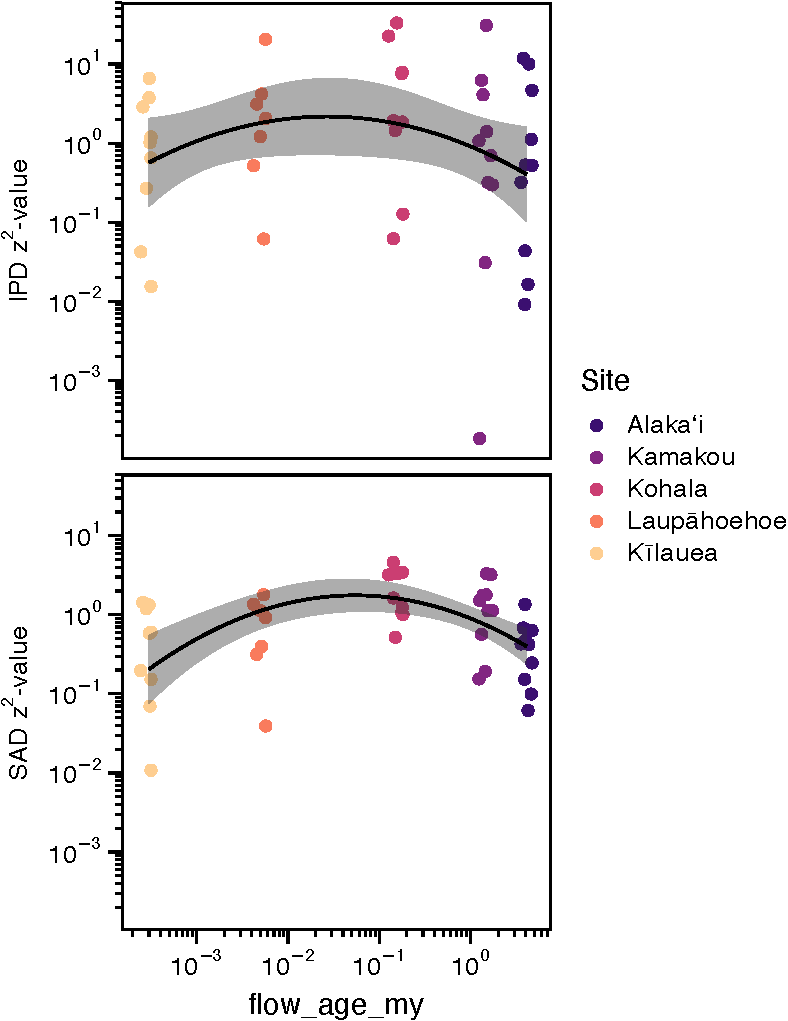
\includegraphics[keepaspectratio]{hawaii-arth-mete-supp_files/figure-pdf/fig-z2-chrono-1.pdf}}

}

\caption{\label{fig-z2-chrono}Deviations from METE as measured by
\(z^2\) across the chronosequence.}

\end{figure}%

\section{How do observed patterns deviate from
METE?}\label{how-do-observed-patterns-deviate-from-mete}

As could be predicted from the analysis of METE deviations across the
chronosequence, generally \(z^2\)-values of the SAD and IPD are
correlated Supplementary Figure~\ref{fig-z2-cor}.

\begin{Shaded}
\begin{Highlighting}[]
\NormalTok{expl }\OtherTok{\textless{}{-}} \FunctionTok{data.frame}\NormalTok{(}\AttributeTok{site =} \FunctionTok{c}\NormalTok{(}\StringTok{"VO"}\NormalTok{, }\StringTok{"KH"}\NormalTok{), }
                   \AttributeTok{site\_name =} \FunctionTok{c}\NormalTok{(}\StringTok{"Kīlauea"}\NormalTok{, }\StringTok{"Kohala"}\NormalTok{),}
                   \AttributeTok{tree =} \FunctionTok{c}\NormalTok{(}\DecValTok{7}\NormalTok{, }\DecValTok{1}\NormalTok{), }
                   \AttributeTok{deviation =} \FunctionTok{c}\NormalTok{(}\StringTok{"lo"}\NormalTok{, }\StringTok{"hi"}\NormalTok{))}


\FunctionTok{ggplot}\NormalTok{(arth\_mete, }\FunctionTok{aes}\NormalTok{(z2\_sad, z2\_ipd, }\AttributeTok{color =}\NormalTok{ site\_name)) }\SpecialCharTok{+}
    \FunctionTok{geom\_point}\NormalTok{() }\SpecialCharTok{+}
    \FunctionTok{geom\_point}\NormalTok{(}\AttributeTok{data =} \FunctionTok{left\_join}\NormalTok{(expl, arth\_mete), }
               \AttributeTok{mapping =} \FunctionTok{aes}\NormalTok{(z2\_sad, z2\_ipd), }
               \AttributeTok{size =} \DecValTok{6}\NormalTok{, }
               \AttributeTok{show.legend =} \ConstantTok{FALSE}\NormalTok{) }\SpecialCharTok{+}
    \FunctionTok{geom\_point}\NormalTok{(}\AttributeTok{data =} \FunctionTok{left\_join}\NormalTok{(expl, arth\_mete), }
               \AttributeTok{mapping =} \FunctionTok{aes}\NormalTok{(z2\_sad, z2\_ipd), }
               \AttributeTok{size =} \DecValTok{6}\NormalTok{, }\AttributeTok{shape =} \DecValTok{1}\NormalTok{, }\AttributeTok{color =} \StringTok{"black"}\NormalTok{,}
               \AttributeTok{stroke =} \FloatTok{1.5}\NormalTok{,}
               \AttributeTok{show.legend =} \ConstantTok{FALSE}\NormalTok{) }\SpecialCharTok{+}
    \FunctionTok{xlab}\NormalTok{(}\FunctionTok{expression}\NormalTok{(}\StringTok{"SAD"}\SpecialCharTok{\textasciitilde{}}\NormalTok{z}\SpecialCharTok{\^{}}\DecValTok{2}\SpecialCharTok{*}\StringTok{"{-}values"}\NormalTok{)) }\SpecialCharTok{+}
    \FunctionTok{ylab}\NormalTok{(}\FunctionTok{expression}\NormalTok{(}\StringTok{"IPD"}\SpecialCharTok{\textasciitilde{}}\NormalTok{z}\SpecialCharTok{\^{}}\DecValTok{2}\SpecialCharTok{*}\StringTok{"{-}values"}\NormalTok{)) }\SpecialCharTok{+}
    \FunctionTok{this\_ms\_look}\NormalTok{(}\AttributeTok{log\_x =} \ConstantTok{TRUE}\NormalTok{, }\AttributeTok{log\_y =} \ConstantTok{TRUE}\NormalTok{)}
\end{Highlighting}
\end{Shaded}

\begin{verbatim}
Joining with `by = join_by(site, site_name, tree)`
Joining with `by = join_by(site, site_name, tree)`
\end{verbatim}

\begin{figure}[H]

\centering{

\pandocbounded{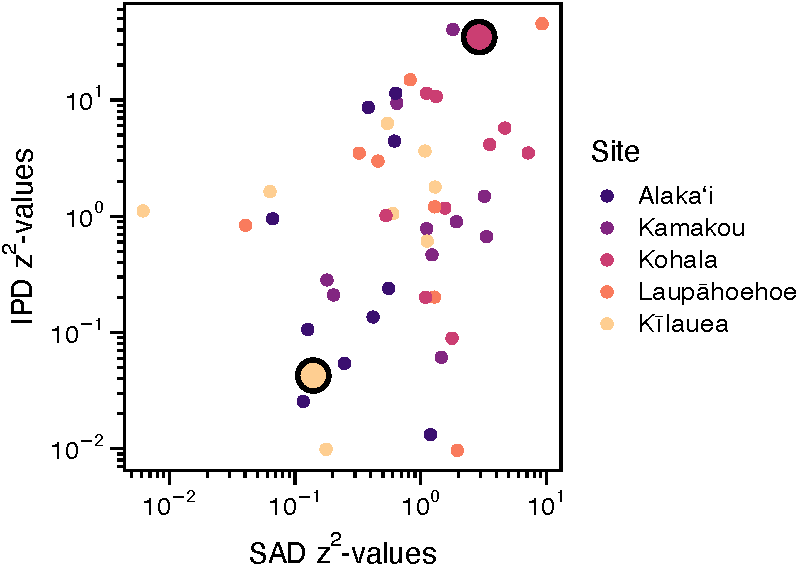
\includegraphics[keepaspectratio]{hawaii-arth-mete-supp_files/figure-pdf/fig-z2-cor-1.pdf}}

}

\caption{\label{fig-z2-cor}Relationship between deviations of SAD and
IPD. Slighlty enlarged, circled points are those used as examples of low
and high deviation from METE}

\end{figure}%

Next we determine how the observed data deviate from the METE
predictions. To begin we look at two exemplar SADs and two exemplar IPDs
representing low and high deviation from METE (Supplementary
Figure~\ref{fig-how-diff}). The high and low \(z^2\)-values of these
samples are highlighted in Supplementary Figure~\ref{fig-z2-cor}.
Specific samples were chosen such that they have comparable state
variables.

\begin{Shaded}
\begin{Highlighting}[]
\CommentTok{\# function to summarize theoretical and observed distributions}
\CommentTok{\# given one sample \textasciigrave{}x\textasciigrave{}}

\NormalTok{mk\_summ }\OtherTok{\textless{}{-}} \ControlFlowTok{function}\NormalTok{(x) \{}
\NormalTok{    esf }\OtherTok{\textless{}{-}} \FunctionTok{meteESF}\NormalTok{(x}\SpecialCharTok{$}\NormalTok{species\_code, x}\SpecialCharTok{$}\NormalTok{abundance, x}\SpecialCharTok{$}\NormalTok{metabolic\_rate)}
    
    \FunctionTok{list}\NormalTok{(}\AttributeTok{sad =} \FunctionTok{sad}\NormalTok{(esf),}
         \AttributeTok{ipd =} \FunctionTok{ipd}\NormalTok{(esf)) }\SpecialCharTok{|\textgreater{}} 
        \FunctionTok{lapply}\NormalTok{(}\ControlFlowTok{function}\NormalTok{(x) \{}
\NormalTok{            thr }\OtherTok{\textless{}{-}} \FunctionTok{samp\_mete}\NormalTok{(x, }\AttributeTok{n =} \DecValTok{1000}\NormalTok{) }\SpecialCharTok{|\textgreater{}} 
                \FunctionTok{summarize\_samp\_mete}\NormalTok{()}
            
\NormalTok{            obs }\OtherTok{\textless{}{-}} \FunctionTok{data.frame}\NormalTok{(}\AttributeTok{rank =} \FunctionTok{seq\_along}\NormalTok{(x}\SpecialCharTok{$}\NormalTok{data), }
                              \AttributeTok{abund\_obs =}\NormalTok{ x}\SpecialCharTok{$}\NormalTok{data)}
            
            \FunctionTok{full\_join}\NormalTok{(thr, obs)}
\NormalTok{        \}) }\SpecialCharTok{|\textgreater{}} 
        \FunctionTok{bind\_rows}\NormalTok{(}\AttributeTok{.id =} \StringTok{"dist"}\NormalTok{)}
\NormalTok{\}}




\NormalTok{expl\_samps }\OtherTok{\textless{}{-}} \FunctionTok{left\_join}\NormalTok{(expl, arth) }\SpecialCharTok{|\textgreater{}} 
\NormalTok{    (\textbackslash{}(x) }\FunctionTok{split}\NormalTok{(x, x}\SpecialCharTok{$}\NormalTok{deviation, }\AttributeTok{drop =} \ConstantTok{TRUE}\NormalTok{))() }\SpecialCharTok{|\textgreater{}} 
    \FunctionTok{lapply}\NormalTok{(mk\_summ) }\SpecialCharTok{|\textgreater{}} 
    \FunctionTok{bind\_rows}\NormalTok{(}\AttributeTok{.id =} \StringTok{"deviation"}\NormalTok{)}
\end{Highlighting}
\end{Shaded}

\begin{verbatim}
Joining with `by = join_by(site, site_name, tree)`
Joining with `by = join_by(rank)`
Joining with `by = join_by(rank)`
Joining with `by = join_by(rank)`
Joining with `by = join_by(rank)`
\end{verbatim}

\begin{Shaded}
\begin{Highlighting}[]
\NormalTok{fig\_how\_diff }\OtherTok{\textless{}{-}} \FunctionTok{ggplot}\NormalTok{(expl\_samps, }\FunctionTok{aes}\NormalTok{(rank, m)) }\SpecialCharTok{+}
    \FunctionTok{geom\_point}\NormalTok{(}\FunctionTok{aes}\NormalTok{(rank, abund\_obs)) }\SpecialCharTok{+}
    \FunctionTok{geom\_ribbon}\NormalTok{(}\FunctionTok{aes}\NormalTok{(}\AttributeTok{ymin =}\NormalTok{ lo, }\AttributeTok{ymax =}\NormalTok{ hi), }
                \AttributeTok{fill =} \StringTok{"\#489BC5"}\NormalTok{, }\AttributeTok{alpha =} \FloatTok{0.75}\NormalTok{) }\SpecialCharTok{+}
    \FunctionTok{geom\_line}\NormalTok{(}\AttributeTok{color =} \StringTok{"\#489BC5"}\NormalTok{) }\SpecialCharTok{+}
    \FunctionTok{facet\_grid2}\NormalTok{(}
        \AttributeTok{rows =} \FunctionTok{vars}\NormalTok{(dist), }\AttributeTok{cols =} \FunctionTok{vars}\NormalTok{(deviation), }
        \AttributeTok{scales =} \StringTok{"free"}\NormalTok{, }\AttributeTok{independent =} \StringTok{"x"}\NormalTok{, }
        \AttributeTok{labeller =} \FunctionTok{as\_labeller}\NormalTok{(}
            \FunctionTok{c}\NormalTok{(}\AttributeTok{hi =} \StringTok{"High deviation"}\NormalTok{, }\AttributeTok{lo =} \StringTok{"Low deviation"}\NormalTok{, }
              \AttributeTok{ipd =} \StringTok{"Metabolic rate"}\NormalTok{, }\AttributeTok{sad =} \StringTok{"Abundance"}\NormalTok{)}
\NormalTok{        ), }
        \AttributeTok{switch =} \StringTok{"y"}
\NormalTok{    ) }\SpecialCharTok{+}
    \FunctionTok{xlab}\NormalTok{(}\StringTok{"Rank"}\NormalTok{) }\SpecialCharTok{+}
    \FunctionTok{ylab}\NormalTok{(}\StringTok{""}\NormalTok{) }\SpecialCharTok{+}
    \FunctionTok{this\_ms\_look}\NormalTok{(}\AttributeTok{log\_y =} \ConstantTok{TRUE}\NormalTok{) }\SpecialCharTok{+}
    \FunctionTok{theme}\NormalTok{(}\AttributeTok{strip.background.y =} \FunctionTok{element\_blank}\NormalTok{(), }
          \AttributeTok{strip.placement.y =} \StringTok{"outside"}\NormalTok{,}
          \AttributeTok{strip.text.y =} \FunctionTok{element\_text}\NormalTok{(}\AttributeTok{size =} \DecValTok{14}\NormalTok{))}

\NormalTok{fig\_how\_diff}
\end{Highlighting}
\end{Shaded}

\begin{figure}[H]

\centering{

\pandocbounded{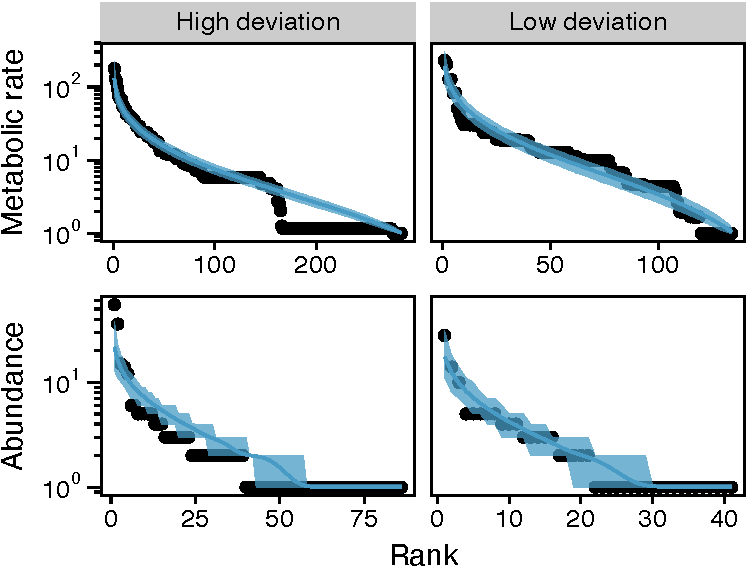
\includegraphics[keepaspectratio]{hawaii-arth-mete-supp_files/figure-pdf/fig-how-diff-1.pdf}}

}

\caption{\label{fig-how-diff}Two exemplar IPDs and SADs showing high and
low deviation from METE. The low deviation distributions come from the
same sample at the Alakaʻi site while the high deviation distributions
come from the same sample at the Kamakou site. Samples were choosen to
represent ranges of deviation while still being similar in state
variables}

\end{figure}%

Looking across all samples (Supplementary Figure~\ref{fig-how-z2}) we
see that deviations between observed and theoretical SADs is
consistently in the direction of under-predicted both rarity and
dominance (i.e.~observed SADs have more rarity and greater dominance
than theoretical predictions). Indeed, only one sample shows a (small)
over-prediction in dominance, and only two samples show a (small)
over-prediction in rarity. This means that observed SADs are more uneven
than the METE prediction.

\begin{Shaded}
\begin{Highlighting}[]
\NormalTok{fig\_how\_z2 }\OtherTok{\textless{}{-}} \FunctionTok{bind\_rows}\NormalTok{(}\AttributeTok{sad =} \FunctionTok{select}\NormalTok{(arth\_mete, site\_name, }
                       \AttributeTok{z2 =}\NormalTok{ z2\_sad, }\AttributeTok{rar\_diff =}\NormalTok{ n1\_diff, }\AttributeTok{dom\_diff =}\NormalTok{ nmax\_diff),}
          \AttributeTok{ipd =} \FunctionTok{select}\NormalTok{(arth\_mete, site\_name, }
                       \AttributeTok{z2 =}\NormalTok{ z2\_ipd, }\AttributeTok{rar\_diff =}\NormalTok{ p1\_diff, }\AttributeTok{dom\_diff =}\NormalTok{ pmax\_diff),}
          \AttributeTok{.id =} \StringTok{"dist"}\NormalTok{) }\SpecialCharTok{|\textgreater{}} 
    \FunctionTok{pivot\_longer}\NormalTok{(}\FunctionTok{ends\_with}\NormalTok{(}\StringTok{"diff"}\NormalTok{), }
                 \AttributeTok{names\_to =} \FunctionTok{c}\NormalTok{(}\StringTok{"comp"}\NormalTok{, }\StringTok{".value"}\NormalTok{), }
                 \AttributeTok{names\_sep =} \StringTok{"\_"}\NormalTok{) }\SpecialCharTok{|\textgreater{}} 
    \FunctionTok{ggplot}\NormalTok{(}\FunctionTok{aes}\NormalTok{(diff, z2, }\AttributeTok{color =}\NormalTok{ site\_name)) }\SpecialCharTok{+}
    \FunctionTok{geom\_point}\NormalTok{() }\SpecialCharTok{+}
    \FunctionTok{facet\_grid2}\NormalTok{(}\AttributeTok{rows =} \FunctionTok{vars}\NormalTok{(dist), }\AttributeTok{cols =} \FunctionTok{vars}\NormalTok{(comp), }
                \AttributeTok{scales =} \StringTok{"free"}\NormalTok{, }\AttributeTok{independent =} \StringTok{"x"}\NormalTok{, }
                \AttributeTok{labeller =} \FunctionTok{as\_labeller}\NormalTok{(}
                    \FunctionTok{c}\NormalTok{(}\AttributeTok{ipd =} \StringTok{"}\SpecialCharTok{\textbackslash{}"}\StringTok{IPD}\SpecialCharTok{\textbackslash{}"}\StringTok{\textasciitilde{}z\^{}2*}\SpecialCharTok{\textbackslash{}"}\StringTok{{-}value}\SpecialCharTok{\textbackslash{}"}\StringTok{"}\NormalTok{, }
                      \AttributeTok{sad =} \StringTok{"}\SpecialCharTok{\textbackslash{}"}\StringTok{SAD}\SpecialCharTok{\textbackslash{}"}\StringTok{\textasciitilde{}z\^{}2*}\SpecialCharTok{\textbackslash{}"}\StringTok{{-}value}\SpecialCharTok{\textbackslash{}"}\StringTok{"}\NormalTok{, }
                      \AttributeTok{dom =} \StringTok{"}\SpecialCharTok{\textbackslash{}"}\StringTok{Diff. in dominance}\SpecialCharTok{\textbackslash{}"}\StringTok{"}\NormalTok{, }
                      \AttributeTok{rar =} \StringTok{"}\SpecialCharTok{\textbackslash{}"}\StringTok{Diff. in rarity}\SpecialCharTok{\textbackslash{}"}\StringTok{"}\NormalTok{),}
\NormalTok{                    label\_parsed}
\NormalTok{                ), }
                \AttributeTok{switch =} \StringTok{"both"}\NormalTok{) }\SpecialCharTok{+}
    \FunctionTok{xlab}\NormalTok{(}\StringTok{""}\NormalTok{) }\SpecialCharTok{+}
    \FunctionTok{ylab}\NormalTok{(}\StringTok{""}\NormalTok{) }\SpecialCharTok{+}
    \FunctionTok{this\_ms\_look}\NormalTok{(}\AttributeTok{log\_y =} \ConstantTok{TRUE}\NormalTok{) }\SpecialCharTok{+}
    \FunctionTok{geom\_vline}\NormalTok{(}\AttributeTok{xintercept =} \DecValTok{0}\NormalTok{, }\AttributeTok{color =} \StringTok{"gray"}\NormalTok{) }\SpecialCharTok{+}
    \FunctionTok{theme}\NormalTok{(}\AttributeTok{strip.background =} \FunctionTok{element\_blank}\NormalTok{(), }
          \AttributeTok{strip.placement =} \StringTok{"outside"}\NormalTok{,}
          \AttributeTok{strip.text.y =} \FunctionTok{element\_text}\NormalTok{(}\AttributeTok{size =} \DecValTok{14}\NormalTok{))}


\NormalTok{fig\_how\_z2}
\end{Highlighting}
\end{Shaded}

\begin{figure}[H]

\centering{

\pandocbounded{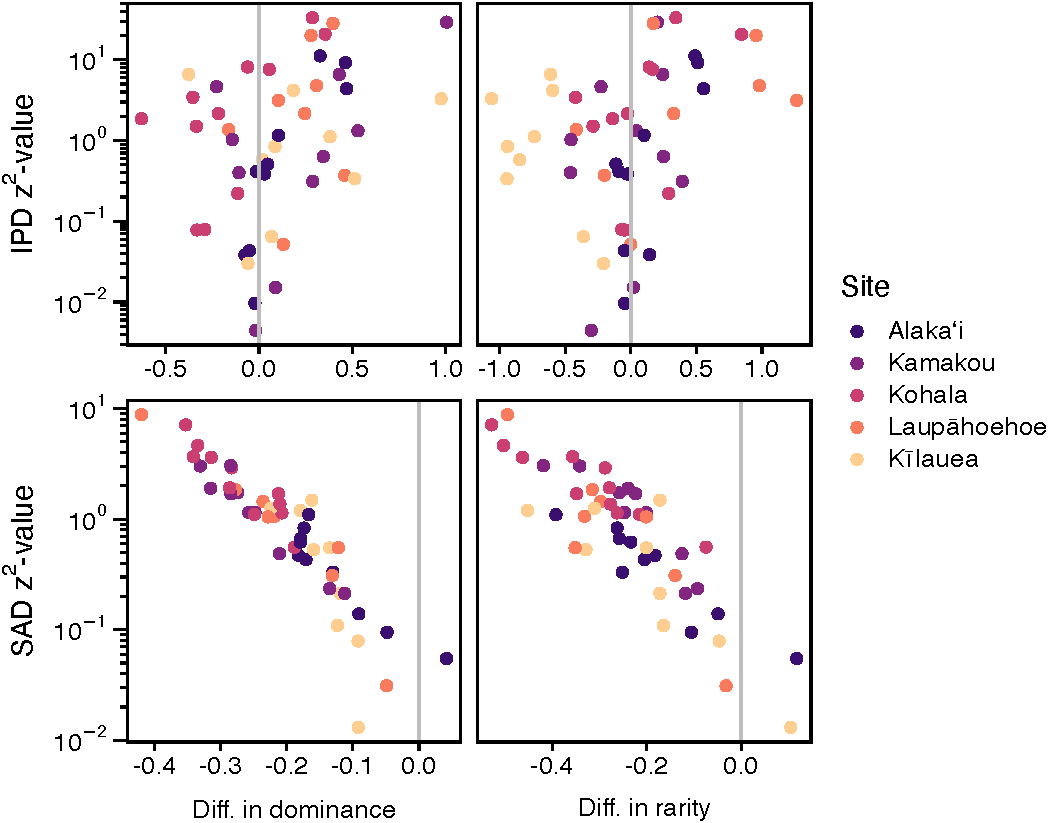
\includegraphics[keepaspectratio]{hawaii-arth-mete-supp_files/figure-pdf/fig-how-z2-1.pdf}}

}

\caption{\label{fig-how-z2}Relationship between \(z^2\) measure of
deviation from METE and different metrics describing how observed data
and METE predictions diverge.}

\end{figure}%

In the case of the IPD dominance refers to metabolic rates of
individuals with the highest metabolic rates, and rarity refers to the
number of individuals with very low metabolic rates. Actual and
theoretical IPDs do not show this consistent discrepancy between
observed and predicted dominance and rarity. To evaluate this we model
the probability of whether the log ratio is above or below zero with an
intercept only binomial GLM.

\begin{Shaded}
\begin{Highlighting}[]
\CommentTok{\# "successes" and "failures" for GLM}
\NormalTok{ipd\_diff }\OtherTok{\textless{}{-}} \FunctionTok{summarize}\NormalTok{(arth\_mete, }
                      \AttributeTok{n\_over\_dom =} \FunctionTok{sum}\NormalTok{(pmax\_diff }\SpecialCharTok{\textless{}} \DecValTok{0}\NormalTok{), }
                      \AttributeTok{n\_undr\_dom =} \FunctionTok{sum}\NormalTok{(pmax\_diff }\SpecialCharTok{\textgreater{}} \DecValTok{0}\NormalTok{), }
                      \AttributeTok{n\_over\_rar =} \FunctionTok{sum}\NormalTok{(p1\_diff }\SpecialCharTok{\textless{}} \DecValTok{0}\NormalTok{), }
                      \AttributeTok{n\_undr\_rar =} \FunctionTok{sum}\NormalTok{(p1\_diff }\SpecialCharTok{\textgreater{}} \DecValTok{0}\NormalTok{), }
                      \AttributeTok{.by =}\NormalTok{ site)}

\CommentTok{\# dominance }
\NormalTok{pmax\_mod }\OtherTok{\textless{}{-}} \FunctionTok{glm}\NormalTok{(}\FunctionTok{cbind}\NormalTok{(n\_over\_dom, n\_undr\_dom) }\SpecialCharTok{\textasciitilde{}} \DecValTok{1}\NormalTok{, }
                \AttributeTok{family =}\NormalTok{ binomial, }\AttributeTok{data =}\NormalTok{ ipd\_diff) }

\FunctionTok{summary}\NormalTok{(pmax\_mod)}
\end{Highlighting}
\end{Shaded}

\begin{verbatim}

Call:
glm(formula = cbind(n_over_dom, n_undr_dom) ~ 1, family = binomial, 
    data = ipd_diff)

Coefficients:
             Estimate Std. Error z value Pr(>|z|)
(Intercept) 5.320e-15  2.887e-01       0        1

(Dispersion parameter for binomial family taken to be 1)

    Null deviance: 8.3371  on 4  degrees of freedom
Residual deviance: 8.3371  on 4  degrees of freedom
AIC: 23.11

Number of Fisher Scoring iterations: 3
\end{verbatim}

\begin{Shaded}
\begin{Highlighting}[]
\CommentTok{\# rarity}
\NormalTok{p1\_mod }\OtherTok{\textless{}{-}} \FunctionTok{glm}\NormalTok{(}\FunctionTok{cbind}\NormalTok{(n\_over\_rar, n\_undr\_rar) }\SpecialCharTok{\textasciitilde{}} \DecValTok{1}\NormalTok{, }
              \AttributeTok{family =}\NormalTok{ binomial, }\AttributeTok{data =}\NormalTok{ ipd\_diff)}

\FunctionTok{summary}\NormalTok{(p1\_mod)}
\end{Highlighting}
\end{Shaded}

\begin{verbatim}

Call:
glm(formula = cbind(n_over_rar, n_undr_rar) ~ 1, family = binomial, 
    data = ipd_diff)

Coefficients:
            Estimate Std. Error z value Pr(>|z|)
(Intercept)  -0.3514     0.2994  -1.173    0.241

(Dispersion parameter for binomial family taken to be 1)

    Null deviance: 14.764  on 4  degrees of freedom
Residual deviance: 14.764  on 4  degrees of freedom
AIC: 28.458

Number of Fisher Scoring iterations: 4
\end{verbatim}

The fact that in both models the intercept is not significantly
different from the null (\(p = 0.5\)) means that there is not evidence
of systematic difference between thertical prediction and observed IPD.

\section{Comparing deviations from METE with potential explanatory
variables}\label{comparing-deviations-from-mete-with-potential-explanatory-variables}

\subsection{Deviation vs.~proportion of non-native
species}\label{deviation-vs.-proportion-of-non-native-species}

To see if proportion of non-native species has any relationship with
deviation from METE we use meta regression as with the chronosequence
analysis. The below code produces this meta regression and tests the
affect of proportion of non-native species on deviations of the SAD and
IPD from METE predictions.

\begin{Shaded}
\begin{Highlighting}[]
\CommentTok{\# calculate proportion of non{-}native spp per site}
\NormalTok{mete\_by\_non }\OtherTok{\textless{}{-}} \FunctionTok{summarize}\NormalTok{(}
\NormalTok{    arth, }
    \AttributeTok{prop\_nspp\_non\_nat =} \FunctionTok{n\_distinct}\NormalTok{(}
\NormalTok{        species\_code[}\SpecialCharTok{!}\NormalTok{(origin }\SpecialCharTok{\%in\%} \FunctionTok{c}\NormalTok{(}\StringTok{"endemic"}\NormalTok{, }\StringTok{"indigneous"}\NormalTok{))]) }\SpecialCharTok{/} 
        \FunctionTok{n\_distinct}\NormalTok{(species\_code),}
    \AttributeTok{.by =}\NormalTok{ site\_name) }\SpecialCharTok{|\textgreater{}} 
    \CommentTok{\# join to mete summary statistics}
    \FunctionTok{full\_join}\NormalTok{(arth\_mete)}
\end{Highlighting}
\end{Shaded}

\begin{verbatim}
Joining with `by = join_by(site_name)`
\end{verbatim}

\begin{Shaded}
\begin{Highlighting}[]
\CommentTok{\# sad regression }
\NormalTok{sad\_rma\_non }\OtherTok{\textless{}{-}} \FunctionTok{site\_means\_lm}\NormalTok{(}\FunctionTok{log}\NormalTok{(z2\_sad) }\SpecialCharTok{\textasciitilde{}}\NormalTok{ prop\_nspp\_non\_nat }\SpecialCharTok{+}\NormalTok{ (}\DecValTok{1} \SpecialCharTok{|}\NormalTok{ site), }
                             \CommentTok{\# excluding Kīlauea site because it is }
                             \CommentTok{\# quite different, further assessed below}
                             \FunctionTok{filter}\NormalTok{(mete\_by\_non, site }\SpecialCharTok{!=} \StringTok{"VO"}\NormalTok{))}

\CommentTok{\# sad likelihood ratio test}
\FunctionTok{anova}\NormalTok{(sad\_rma\_non)}
\end{Highlighting}
\end{Shaded}

\begin{verbatim}

Test of Moderators (coefficient 2):
QM(df = 1) = 22.3287, p-val < .0001
\end{verbatim}

\begin{Shaded}
\begin{Highlighting}[]
\CommentTok{\# ipd regression }
\NormalTok{ipd\_rma\_non }\OtherTok{\textless{}{-}} \FunctionTok{site\_means\_lm}\NormalTok{(}\FunctionTok{log}\NormalTok{(z2\_ipd) }\SpecialCharTok{\textasciitilde{}}\NormalTok{ prop\_nspp\_non\_nat }\SpecialCharTok{+}\NormalTok{ (}\DecValTok{1} \SpecialCharTok{|}\NormalTok{ site), }
                             \CommentTok{\# excluding Kīlauea site}
                             \FunctionTok{filter}\NormalTok{(mete\_by\_non, site }\SpecialCharTok{!=} \StringTok{"VO"}\NormalTok{))}

\CommentTok{\# ipd likelihood ratio test}
\FunctionTok{anova}\NormalTok{(ipd\_rma\_non)}
\end{Highlighting}
\end{Shaded}

\begin{verbatim}

Test of Moderators (coefficient 2):
QM(df = 1) = 5.2616, p-val = 0.0218
\end{verbatim}

The below code is used for visualizing the results. Note that Kīlauea is
considered separately because it falls clearly below the expected trend
based on other sites. In the case of the SAD, the mean and 95\% CI of
the \(z^2\)-value for Kīlauea is below both the expected value and 95\%
CI of the rest of the data. In the case of the Kīlauea IPD only the mean
of \(z^2\)-values is below the 95\% CI of the rest of the data; the two
CIs do overlap. This is why in the meta regression analysis Kīlauea was
excluded, so we could interrogate the way it deviates from the overall
pattern.

\begin{Shaded}
\begin{Highlighting}[]
\CommentTok{\# 95\% CI for mean of Kīlauea site}
\NormalTok{vo\_mean }\OtherTok{\textless{}{-}} \FunctionTok{filter}\NormalTok{(mete\_by\_non, site }\SpecialCharTok{==} \StringTok{"VO"}\NormalTok{) }\SpecialCharTok{|\textgreater{}} 
    \FunctionTok{pivot\_longer}\NormalTok{(}\FunctionTok{starts\_with}\NormalTok{(}\StringTok{"z2"}\NormalTok{), }
                 \AttributeTok{names\_to =} \FunctionTok{c}\NormalTok{(}\StringTok{".value"}\NormalTok{, }\StringTok{"dist"}\NormalTok{), }\AttributeTok{names\_sep =} \StringTok{"\_"}\NormalTok{) }\SpecialCharTok{|\textgreater{}} 
    \FunctionTok{mutate}\NormalTok{(}\AttributeTok{z2 =} \FunctionTok{log}\NormalTok{(z2)) }\SpecialCharTok{|\textgreater{}} 
    \FunctionTok{summarize}\NormalTok{(}\AttributeTok{site\_name =} \FunctionTok{first}\NormalTok{(site\_name), }
              \AttributeTok{prop\_nspp\_non\_nat =} \FunctionTok{mean}\NormalTok{(prop\_nspp\_non\_nat),}
              \AttributeTok{z2\_mean =} \FunctionTok{mean}\NormalTok{(z2), }
              \AttributeTok{z2\_se =} \FunctionTok{sd}\NormalTok{(z2) }\SpecialCharTok{/} \FunctionTok{sqrt}\NormalTok{(}\FunctionTok{n}\NormalTok{()), }
              \AttributeTok{z2\_lo =}\NormalTok{ z2\_mean }\SpecialCharTok{{-}} \FloatTok{1.96} \SpecialCharTok{*}\NormalTok{ z2\_se,}
              \AttributeTok{z2\_hi =}\NormalTok{ z2\_mean }\SpecialCharTok{+} \FloatTok{1.96} \SpecialCharTok{*}\NormalTok{ z2\_se, }
              \AttributeTok{.by =}\NormalTok{ dist) }\SpecialCharTok{|\textgreater{}} 
    \FunctionTok{rename}\NormalTok{(}\AttributeTok{z2 =}\NormalTok{ z2\_mean) }\SpecialCharTok{|\textgreater{}} 
    \FunctionTok{mutate}\NormalTok{(}\FunctionTok{across}\NormalTok{(}\FunctionTok{starts\_with}\NormalTok{(}\StringTok{"z2"}\NormalTok{), exp))}

\CommentTok{\# prediction for plotting}
\NormalTok{x }\OtherTok{\textless{}{-}} \FunctionTok{range}\NormalTok{(mete\_by\_non}\SpecialCharTok{$}\NormalTok{prop\_nspp\_non\_nat) }\SpecialCharTok{|\textgreater{}} 
\NormalTok{    (\textbackslash{}(x) }\FunctionTok{seq}\NormalTok{(x[}\DecValTok{1}\NormalTok{], x[}\DecValTok{2}\NormalTok{], }\AttributeTok{length.out =} \DecValTok{50}\NormalTok{))() }\SpecialCharTok{|\textgreater{}} 
    \FunctionTok{data.frame}\NormalTok{(}\AttributeTok{prop\_nspp\_non\_nat =}\NormalTok{ \_)}

\NormalTok{sad\_hat }\OtherTok{\textless{}{-}} \FunctionTok{site\_means\_predict}\NormalTok{(sad\_rma\_non, }\AttributeTok{newdata =}\NormalTok{ x)}
\NormalTok{ipd\_hat }\OtherTok{\textless{}{-}} \FunctionTok{site\_means\_predict}\NormalTok{(ipd\_rma\_non, }\AttributeTok{newdata =}\NormalTok{ x)}

\NormalTok{z2\_non\_pred }\OtherTok{\textless{}{-}} \FunctionTok{bind\_rows}\NormalTok{(}\AttributeTok{sad =} \FunctionTok{data.frame}\NormalTok{(x, sad\_hat), }
                         \AttributeTok{ipd =} \FunctionTok{data.frame}\NormalTok{(x, ipd\_hat), }
                         \AttributeTok{.id =} \StringTok{"dist"}\NormalTok{) }\SpecialCharTok{|\textgreater{}} 
    \FunctionTok{select}\NormalTok{(}\SpecialCharTok{!}\NormalTok{se) }\SpecialCharTok{|\textgreater{}} 
    \FunctionTok{rename}\NormalTok{(}\AttributeTok{z2 =}\NormalTok{ pred,}
           \AttributeTok{z2\_lo =}\NormalTok{ ci.lb, }
           \AttributeTok{z2\_hi =}\NormalTok{ ci.ub) }\SpecialCharTok{|\textgreater{}} 
    \FunctionTok{mutate}\NormalTok{(}\FunctionTok{across}\NormalTok{(}\FunctionTok{starts\_with}\NormalTok{(}\StringTok{"z2"}\NormalTok{), exp))}

\CommentTok{\# plotting}
\NormalTok{fig\_dev\_non }\OtherTok{\textless{}{-}} \FunctionTok{pivot\_longer}\NormalTok{(mete\_by\_non, }\FunctionTok{starts\_with}\NormalTok{(}\StringTok{"z2"}\NormalTok{), }
                            \AttributeTok{names\_to =} \FunctionTok{c}\NormalTok{(}\StringTok{".value"}\NormalTok{, }\StringTok{"dist"}\NormalTok{), }
                            \AttributeTok{names\_sep =} \StringTok{"\_"}\NormalTok{) }\SpecialCharTok{|\textgreater{}} 
    \FunctionTok{ggplot}\NormalTok{(}\FunctionTok{aes}\NormalTok{(prop\_nspp\_non\_nat, z2, }\AttributeTok{color =}\NormalTok{ site\_name)) }\SpecialCharTok{+}
    \FunctionTok{geom\_jitter}\NormalTok{(}\AttributeTok{width =} \FloatTok{0.002}\NormalTok{) }\SpecialCharTok{+}
    \CommentTok{\# confidence envelope}
    \FunctionTok{geom\_ribbon}\NormalTok{(}\AttributeTok{data =}\NormalTok{ z2\_non\_pred, }
                \AttributeTok{mapping =} \FunctionTok{aes}\NormalTok{(}\AttributeTok{x =}\NormalTok{ prop\_nspp\_non\_nat, }
                              \AttributeTok{ymin =}\NormalTok{ z2\_lo, }
                              \AttributeTok{ymax =}\NormalTok{ z2\_hi), }
                \AttributeTok{color =} \StringTok{"transparent"}\NormalTok{, }\AttributeTok{alpha =} \FloatTok{0.4}\NormalTok{) }\SpecialCharTok{+}
    \CommentTok{\# central tendency }
    \FunctionTok{geom\_line}\NormalTok{(}\AttributeTok{data =}\NormalTok{ z2\_non\_pred, }
              \AttributeTok{mapping =} \FunctionTok{aes}\NormalTok{(prop\_nspp\_non\_nat, z2), }
              \AttributeTok{color =} \StringTok{"black"}\NormalTok{) }\SpecialCharTok{+}
    \FunctionTok{geom\_rect}\NormalTok{(}\AttributeTok{data =}\NormalTok{ vo\_mean, }
              \AttributeTok{mapping =} \FunctionTok{aes}\NormalTok{(}\AttributeTok{xmin =}\NormalTok{ prop\_nspp\_non\_nat }\SpecialCharTok{{-}} \FloatTok{0.002}\NormalTok{, }
                            \AttributeTok{xmax =}\NormalTok{ prop\_nspp\_non\_nat }\SpecialCharTok{+} \FloatTok{0.002}\NormalTok{, }
                            \AttributeTok{ymin =}\NormalTok{ z2\_lo, }
                            \AttributeTok{ymax =}\NormalTok{ z2\_hi), }
              \AttributeTok{color =} \StringTok{"transparent"}\NormalTok{, }\AttributeTok{alpha =} \FloatTok{0.4}\NormalTok{) }\SpecialCharTok{+}
    \FunctionTok{geom\_segment}\NormalTok{(}\AttributeTok{data =}\NormalTok{ vo\_mean, }
              \AttributeTok{mapping =} \FunctionTok{aes}\NormalTok{(}\AttributeTok{x =}\NormalTok{ prop\_nspp\_non\_nat }\SpecialCharTok{{-}} \FloatTok{0.002}\NormalTok{, }
                            \AttributeTok{xend =}\NormalTok{ prop\_nspp\_non\_nat }\SpecialCharTok{+} \FloatTok{0.002}\NormalTok{, }
                            \AttributeTok{y =}\NormalTok{ z2, }
                            \AttributeTok{yend =}\NormalTok{ z2), }
              \AttributeTok{color =} \StringTok{"black"}\NormalTok{) }\SpecialCharTok{+}
    \FunctionTok{facet\_grid}\NormalTok{(}\AttributeTok{rows =} \FunctionTok{vars}\NormalTok{(dist), }
               \AttributeTok{labeller =} \FunctionTok{as\_labeller}\NormalTok{(}
                   \FunctionTok{c}\NormalTok{(}\AttributeTok{ipd =} \StringTok{"}\SpecialCharTok{\textbackslash{}"}\StringTok{IPD}\SpecialCharTok{\textbackslash{}"}\StringTok{\textasciitilde{}z\^{}2*}\SpecialCharTok{\textbackslash{}"}\StringTok{{-}value}\SpecialCharTok{\textbackslash{}"}\StringTok{"}\NormalTok{, }
                     \AttributeTok{sad =} \StringTok{"}\SpecialCharTok{\textbackslash{}"}\StringTok{SAD}\SpecialCharTok{\textbackslash{}"}\StringTok{\textasciitilde{}z\^{}2*}\SpecialCharTok{\textbackslash{}"}\StringTok{{-}value}\SpecialCharTok{\textbackslash{}"}\StringTok{"}\NormalTok{),}
\NormalTok{                   label\_parsed}
\NormalTok{               ), }
               \AttributeTok{switch =} \StringTok{"y"}\NormalTok{) }\SpecialCharTok{+}
    \FunctionTok{xlab}\NormalTok{(}\StringTok{"Proportion of non{-}native spp."}\NormalTok{) }\SpecialCharTok{+}
    \FunctionTok{this\_ms\_look}\NormalTok{(}\AttributeTok{log\_y =} \ConstantTok{TRUE}\NormalTok{) }\SpecialCharTok{+}
    \FunctionTok{theme}\NormalTok{(}\AttributeTok{axis.title.y =} \FunctionTok{element\_blank}\NormalTok{(),}
          \AttributeTok{strip.background =} \FunctionTok{element\_blank}\NormalTok{(), }
          \AttributeTok{strip.placement =} \StringTok{"outside"}\NormalTok{)}



\NormalTok{fig\_dev\_non}
\end{Highlighting}
\end{Shaded}

\begin{figure}[H]

\centering{

\pandocbounded{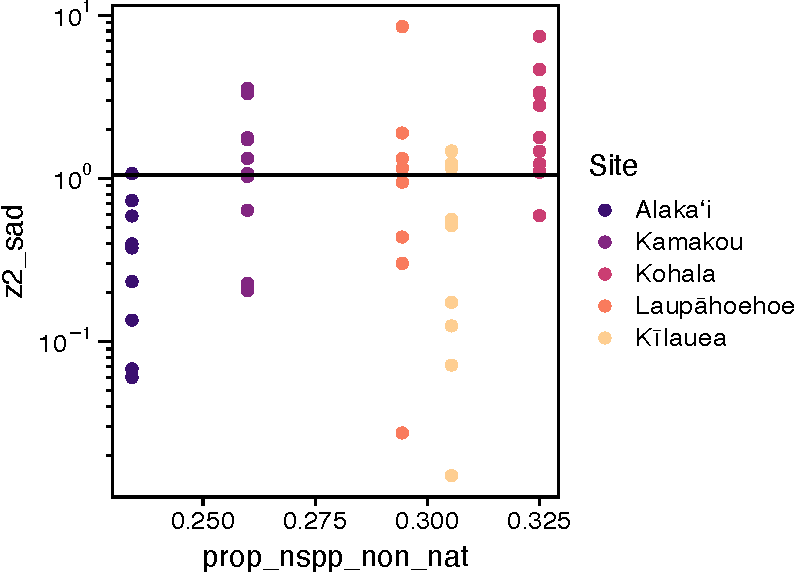
\includegraphics[keepaspectratio]{hawaii-arth-mete-supp_files/figure-pdf/fig-dev-non-1.pdf}}

}

\caption{\label{fig-dev-non}Relationship between proportion of
non-native species and deviation from METE. Kīlauea was excluded from
the overall analysis to be able to compare it separately to the overall
trend. Gray regreions represent 95\% confidence envelopes (or confidence
interval for Kīlauea) and solid lines are expected values.}

\end{figure}%

\subsection{Deviation
vs.~dissimilarity}\label{deviation-vs.-dissimilarity}

We also conducted meta regression to see if \(z^2\)-values change
meaningfully across different levels of within-site, between-sample
dissimilarity or \(\beta\)-diversity. The below code runs this meta
regression analysis.

\begin{Shaded}
\begin{Highlighting}[]
\CommentTok{\# calculate dissimilarity z{-}scores}
\NormalTok{diss }\OtherTok{\textless{}{-}} \FunctionTok{split}\NormalTok{(arth, arth}\SpecialCharTok{$}\NormalTok{site) }\SpecialCharTok{|\textgreater{}} 
    \FunctionTok{sapply}\NormalTok{(}\AttributeTok{FUN =} \ControlFlowTok{function}\NormalTok{(dat) \{}
        \FunctionTok{summarize}\NormalTok{(dat, }\AttributeTok{abund =} \FunctionTok{n}\NormalTok{(), }\AttributeTok{.by =} \FunctionTok{c}\NormalTok{(tree, species\_code)) }\SpecialCharTok{|\textgreater{}} 
            \FunctionTok{pivot\_wider}\NormalTok{(}\AttributeTok{names\_from =}\NormalTok{ species\_code, }
                        \AttributeTok{values\_from =}\NormalTok{ abund, }
                        \AttributeTok{values\_fill =} \DecValTok{0}\NormalTok{) }\SpecialCharTok{|\textgreater{}} 
            \FunctionTok{select}\NormalTok{(}\SpecialCharTok{!}\NormalTok{tree) }\SpecialCharTok{|\textgreater{}} 
            \FunctionTok{bray\_diss\_z}\NormalTok{() }
\NormalTok{    \})}

\CommentTok{\# combine with mete summary statistics}
\NormalTok{mete\_by\_diss }\OtherTok{\textless{}{-}} \FunctionTok{mutate}\NormalTok{(arth\_mete, }
                       \AttributeTok{mean\_diss =}\NormalTok{ diss[site])}


\CommentTok{\# sad regression }
\NormalTok{sad\_rma\_diss }\OtherTok{\textless{}{-}} \FunctionTok{site\_means\_lm}\NormalTok{(}\FunctionTok{log}\NormalTok{(z2\_sad) }\SpecialCharTok{\textasciitilde{}}\NormalTok{ mean\_diss }\SpecialCharTok{+}\NormalTok{ (}\DecValTok{1} \SpecialCharTok{|}\NormalTok{ site),}
                              \AttributeTok{data =}\NormalTok{ mete\_by\_diss)}

\CommentTok{\# sad likelihood ratio test}
\FunctionTok{anova}\NormalTok{(sad\_rma\_diss)}
\end{Highlighting}
\end{Shaded}

\begin{verbatim}

Test of Moderators (coefficient 2):
QM(df = 1) = 29.9678, p-val < .0001
\end{verbatim}

\begin{Shaded}
\begin{Highlighting}[]
\CommentTok{\# ipd regression }
\NormalTok{ipd\_rma\_diss }\OtherTok{\textless{}{-}} \FunctionTok{site\_means\_lm}\NormalTok{(}\FunctionTok{log}\NormalTok{(z2\_ipd) }\SpecialCharTok{\textasciitilde{}}\NormalTok{ mean\_diss }\SpecialCharTok{+}\NormalTok{ (}\DecValTok{1} \SpecialCharTok{|}\NormalTok{ site),}
                              \AttributeTok{data =}\NormalTok{ mete\_by\_diss)}

\CommentTok{\# ipd likelihood ratio test}
\FunctionTok{anova}\NormalTok{(ipd\_rma\_diss)}
\end{Highlighting}
\end{Shaded}

\begin{verbatim}

Test of Moderators (coefficient 2):
QM(df = 1) = 5.4708, p-val = 0.0193
\end{verbatim}

The relationship between deviation from METE and dissimilarity is more
clearly linear than that of proportion non-native species and deviation
from METE. It is therefore worth figuring out if the ways that native
and non-native taxa contribute to dissimilarity is different across
sites.

The below code visualizes the results of the meta regression or SAD and
IPD \(z^2\)-values against dissimilarity.

\begin{Shaded}
\begin{Highlighting}[]
\CommentTok{\# prediction for plotting}
\NormalTok{x }\OtherTok{\textless{}{-}} \FunctionTok{range}\NormalTok{(mete\_by\_diss}\SpecialCharTok{$}\NormalTok{mean\_diss) }\SpecialCharTok{|\textgreater{}} 
\NormalTok{    (\textbackslash{}(x) }\FunctionTok{seq}\NormalTok{(x[}\DecValTok{1}\NormalTok{], x[}\DecValTok{2}\NormalTok{], }\AttributeTok{length.out =} \DecValTok{50}\NormalTok{))() }\SpecialCharTok{|\textgreater{}} 
    \FunctionTok{data.frame}\NormalTok{(}\AttributeTok{mean\_diss =}\NormalTok{ \_)}

\NormalTok{sad\_hat }\OtherTok{\textless{}{-}} \FunctionTok{site\_means\_predict}\NormalTok{(sad\_rma\_diss, }\AttributeTok{newdata =}\NormalTok{ x)}
\NormalTok{ipd\_hat }\OtherTok{\textless{}{-}} \FunctionTok{site\_means\_predict}\NormalTok{(ipd\_rma\_diss, }\AttributeTok{newdata =}\NormalTok{ x)}

\NormalTok{z2\_diss\_pred }\OtherTok{\textless{}{-}} \FunctionTok{bind\_rows}\NormalTok{(}\AttributeTok{sad =} \FunctionTok{data.frame}\NormalTok{(x, sad\_hat), }
                         \AttributeTok{ipd =} \FunctionTok{data.frame}\NormalTok{(x, ipd\_hat), }
                         \AttributeTok{.id =} \StringTok{"dist"}\NormalTok{) }\SpecialCharTok{|\textgreater{}} 
    \FunctionTok{select}\NormalTok{(}\SpecialCharTok{!}\NormalTok{se) }\SpecialCharTok{|\textgreater{}} 
    \FunctionTok{rename}\NormalTok{(}\AttributeTok{z2 =}\NormalTok{ pred,}
           \AttributeTok{z2\_lo =}\NormalTok{ ci.lb, }
           \AttributeTok{z2\_hi =}\NormalTok{ ci.ub) }\SpecialCharTok{|\textgreater{}} 
    \FunctionTok{mutate}\NormalTok{(}\FunctionTok{across}\NormalTok{(}\FunctionTok{starts\_with}\NormalTok{(}\StringTok{"z2"}\NormalTok{), exp))}

\CommentTok{\# plotting}
\NormalTok{fig\_diss\_z }\OtherTok{\textless{}{-}} \FunctionTok{pivot\_longer}\NormalTok{(mete\_by\_diss, }\FunctionTok{starts\_with}\NormalTok{(}\StringTok{"z2"}\NormalTok{), }
                           \AttributeTok{names\_to =} \FunctionTok{c}\NormalTok{(}\StringTok{".value"}\NormalTok{, }\StringTok{"dist"}\NormalTok{), }
                           \AttributeTok{names\_sep =} \StringTok{"\_"}\NormalTok{) }\SpecialCharTok{|\textgreater{}} 
    \FunctionTok{ggplot}\NormalTok{(}\FunctionTok{aes}\NormalTok{(mean\_diss, z2, }\AttributeTok{color =}\NormalTok{ site\_name)) }\SpecialCharTok{+}
    \FunctionTok{geom\_jitter}\NormalTok{(}\AttributeTok{width =} \FloatTok{0.1}\NormalTok{) }\SpecialCharTok{+}
    \CommentTok{\# confidence envelope}
    \FunctionTok{geom\_ribbon}\NormalTok{(}\AttributeTok{data =}\NormalTok{ z2\_diss\_pred, }
                \AttributeTok{mapping =} \FunctionTok{aes}\NormalTok{(}\AttributeTok{x =}\NormalTok{ mean\_diss, }
                              \AttributeTok{ymin =}\NormalTok{ z2\_lo, }
                              \AttributeTok{ymax =}\NormalTok{ z2\_hi), }
                \AttributeTok{color =} \StringTok{"transparent"}\NormalTok{, }\AttributeTok{alpha =} \FloatTok{0.4}\NormalTok{) }\SpecialCharTok{+}
    \CommentTok{\# central tendency }
    \FunctionTok{geom\_line}\NormalTok{(}\AttributeTok{data =}\NormalTok{ z2\_diss\_pred, }
              \AttributeTok{mapping =} \FunctionTok{aes}\NormalTok{(mean\_diss, z2), }
              \AttributeTok{color =} \StringTok{"black"}\NormalTok{) }\SpecialCharTok{+}
    \FunctionTok{facet\_grid}\NormalTok{(}\AttributeTok{rows =} \FunctionTok{vars}\NormalTok{(dist), }
               \AttributeTok{labeller =} \FunctionTok{as\_labeller}\NormalTok{(}
                   \FunctionTok{c}\NormalTok{(}\AttributeTok{ipd =} \StringTok{"}\SpecialCharTok{\textbackslash{}"}\StringTok{IPD}\SpecialCharTok{\textbackslash{}"}\StringTok{\textasciitilde{}z\^{}2*}\SpecialCharTok{\textbackslash{}"}\StringTok{{-}value}\SpecialCharTok{\textbackslash{}"}\StringTok{"}\NormalTok{, }
                     \AttributeTok{sad =} \StringTok{"}\SpecialCharTok{\textbackslash{}"}\StringTok{SAD}\SpecialCharTok{\textbackslash{}"}\StringTok{\textasciitilde{}z\^{}2*}\SpecialCharTok{\textbackslash{}"}\StringTok{{-}value}\SpecialCharTok{\textbackslash{}"}\StringTok{"}\NormalTok{),}
\NormalTok{                   label\_parsed}
\NormalTok{               ), }
               \AttributeTok{switch =} \StringTok{"y"}\NormalTok{) }\SpecialCharTok{+}
    \FunctionTok{xlab}\NormalTok{(}\StringTok{"Mean dissimilarity"}\NormalTok{) }\SpecialCharTok{+}
    \FunctionTok{this\_ms\_look}\NormalTok{(}\AttributeTok{log\_y =} \ConstantTok{TRUE}\NormalTok{) }\SpecialCharTok{+}
    \FunctionTok{theme}\NormalTok{(}\AttributeTok{axis.title.y =} \FunctionTok{element\_blank}\NormalTok{(),}
          \AttributeTok{strip.background =} \FunctionTok{element\_blank}\NormalTok{(), }
          \AttributeTok{strip.placement =} \StringTok{"outside"}\NormalTok{)}

\NormalTok{fig\_diss\_z}
\end{Highlighting}
\end{Shaded}

\begin{figure}[H]

\centering{

\pandocbounded{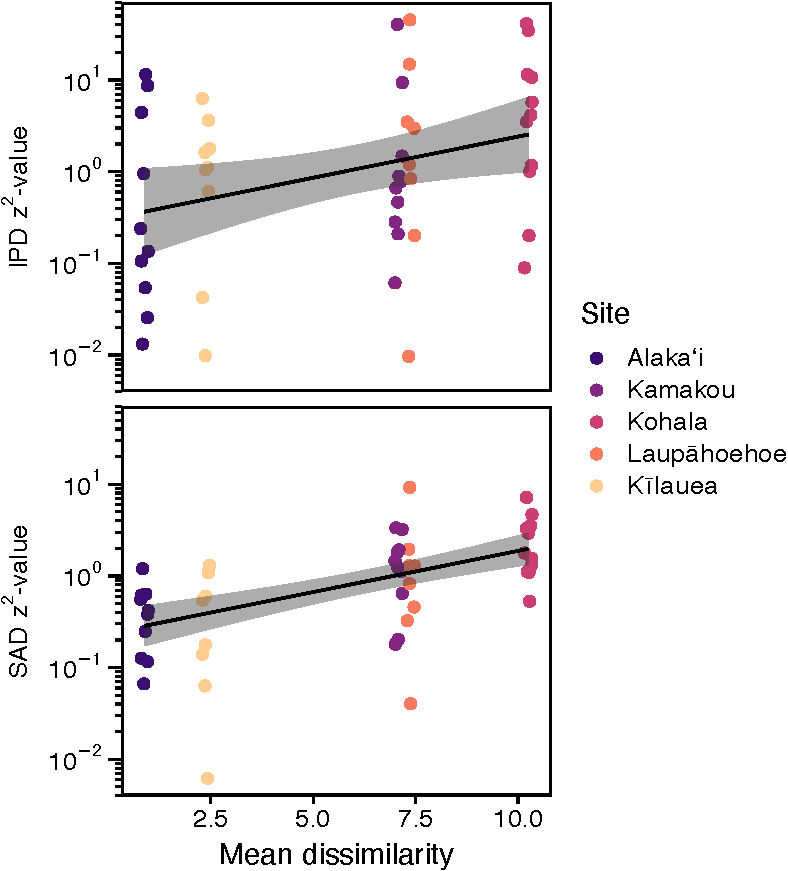
\includegraphics[keepaspectratio]{hawaii-arth-mete-supp_files/figure-pdf/fig-diss-z-1.pdf}}

}

\caption{\label{fig-diss-z}Relationship between dissimilarity and
deviation from METE. Gray regreions represent 95\% confidence envelopes
and solid lines are expected values.}

\end{figure}%

\subsection{Partitioning Bray Curtis dissimilarity between native and
non-native
species}\label{partitioning-bray-curtis-dissimilarity-between-native-and-non-native-species}

To do that we take advantage of the additive nature of Bray Curtis
dissimilarity. Bray Curtis dissimilarity is defined as

\[
d_{kj} = \frac{\sum_i |x_{ij} - x_{ik}|}{\sum_{ij} x_{ij} + x_{ik}}
\]

where \(x_{ij}\) and \(x_{ik}\) are the abundances of species \(i\) at
sites \(j\) and \(k\). This can be partitioned across any grouping of
species, say \((a)\) and \((b)\) with abundances \(x_{ij}^{(a)}\) and
\(x_{ij}^{(b)}\)

\[
d_{kj} = \frac{\sum_i |x_{ij}^{(a)} - x_{ik}^{(a)}|}{\sum_{ij} x_{ij} + x_{ik}} + \frac{\sum_i |x_{ij}^{(b)} - x_{ik}^{(b)}|}{\sum_{ij} x_{ij} + x_{ik}}
\]

Now we can look separately at the contribution of group \((a)\) and
group \((b)\) to the overall dissimilarity. We use this approach to
compare the contributions of native and non-native taxa to overall
dissimilarity. We again make use of a permutational null model to
compare these contributions. This null model cannot be the same as the
null model used to calculate z scores for overall dissimilarity because
that null model shuffled species across samples and individuals across
species. Instead, we want to shuffle group labels (native or non-native)
across species. The custom function \texttt{bray\_part\_z} calculates
these z scores using another custom function \texttt{cswap} from
\emph{HawaiiArthMETE}.

\begin{Shaded}
\begin{Highlighting}[]
\NormalTok{site\_bray\_z }\OtherTok{\textless{}{-}} \FunctionTok{split}\NormalTok{(arth, arth}\SpecialCharTok{$}\NormalTok{site\_name) }\SpecialCharTok{|\textgreater{}} 
    \FunctionTok{lapply}\NormalTok{(}\ControlFlowTok{function}\NormalTok{(dat) \{}
\NormalTok{        comm }\OtherTok{\textless{}{-}} \FunctionTok{summarize}\NormalTok{(dat, }
                  \AttributeTok{abund =} \FunctionTok{n}\NormalTok{(), }
                  \AttributeTok{.by =} \FunctionTok{c}\NormalTok{(tree, species\_code)) }\SpecialCharTok{|\textgreater{}} 
            \FunctionTok{pivot\_wider}\NormalTok{(}\AttributeTok{names\_from =}\NormalTok{ species\_code, }
                        \AttributeTok{values\_from =}\NormalTok{ abund, }
                        \AttributeTok{values\_fill =} \DecValTok{0}\NormalTok{) }\SpecialCharTok{|\textgreater{}} 
            \FunctionTok{select}\NormalTok{(}\SpecialCharTok{!}\NormalTok{tree)}
\NormalTok{        g }\OtherTok{\textless{}{-}}\NormalTok{ dat}\SpecialCharTok{$}\NormalTok{origin[}\FunctionTok{match}\NormalTok{(}\FunctionTok{names}\NormalTok{(comm), dat}\SpecialCharTok{$}\NormalTok{species\_code)] }\SpecialCharTok{\%in\%} 
            \FunctionTok{c}\NormalTok{(}\StringTok{"endemic"}\NormalTok{, }\StringTok{"indigenous"}\NormalTok{)}
        
        \FunctionTok{data.frame}\NormalTok{(}\AttributeTok{bp =} \FunctionTok{bray\_part\_z}\NormalTok{(}\FunctionTok{as.matrix}\NormalTok{(comm), g))}
\NormalTok{    \}) }\SpecialCharTok{|\textgreater{}} 
    \FunctionTok{bind\_rows}\NormalTok{(}\AttributeTok{.id =} \StringTok{"site\_name"}\NormalTok{)}
\end{Highlighting}
\end{Shaded}

Now we can visualize different contributions of native and non-native
species to within-site, between-sample dissimilarity.

\begin{Shaded}
\begin{Highlighting}[]
\NormalTok{site\_bray\_z}\SpecialCharTok{$}\NormalTok{site\_name }\OtherTok{\textless{}{-}} \FunctionTok{factor}\NormalTok{(site\_bray\_z}\SpecialCharTok{$}\NormalTok{site\_name, }
                                \AttributeTok{levels =} \FunctionTok{levels}\NormalTok{(arth}\SpecialCharTok{$}\NormalTok{site\_name))}

\NormalTok{fig\_bray\_part }\OtherTok{\textless{}{-}} \FunctionTok{ggplot}\NormalTok{(}\FunctionTok{arrange}\NormalTok{(site\_bray\_z, }\FunctionTok{as.numeric}\NormalTok{(site\_name)), }
                        \FunctionTok{aes}\NormalTok{(bp, site\_name, }\AttributeTok{fill =}\NormalTok{ site\_name)) }\SpecialCharTok{+}
    \FunctionTok{geom\_bar}\NormalTok{(}\AttributeTok{stat =} \StringTok{"identity"}\NormalTok{) }\SpecialCharTok{+}
    \FunctionTok{this\_ms\_look}\NormalTok{() }\SpecialCharTok{+}
    \FunctionTok{geom\_vline}\NormalTok{(}\AttributeTok{xintercept =} \DecValTok{0}\NormalTok{, }\AttributeTok{color =} \StringTok{"gray"}\NormalTok{) }\SpecialCharTok{+}
    \FunctionTok{xlim}\NormalTok{(}\FunctionTok{c}\NormalTok{(}\SpecialCharTok{{-}}\DecValTok{1}\NormalTok{, }\DecValTok{1}\NormalTok{) }\SpecialCharTok{*} \FunctionTok{max}\NormalTok{(}\FunctionTok{abs}\NormalTok{(site\_bray\_z}\SpecialCharTok{$}\NormalTok{bp))) }\SpecialCharTok{+}
    \FunctionTok{ylab}\NormalTok{(}\StringTok{""}\NormalTok{) }\SpecialCharTok{+}
    \FunctionTok{xlab}\NormalTok{(}\StringTok{"Log ratio dissimilarity partition"}\NormalTok{) }\SpecialCharTok{+}
    \FunctionTok{annotate}\NormalTok{(}\StringTok{"segment"}\NormalTok{, }\AttributeTok{x =} \FunctionTok{c}\NormalTok{(}\SpecialCharTok{{-}}\FloatTok{0.5}\NormalTok{, }\FloatTok{0.5}\NormalTok{), }\AttributeTok{xend =} \FunctionTok{c}\NormalTok{(}\SpecialCharTok{{-}}\FloatTok{2.75}\NormalTok{, }\FloatTok{2.75}\NormalTok{), }
             \AttributeTok{y =} \DecValTok{6}\NormalTok{, }\AttributeTok{yend =} \DecValTok{6}\NormalTok{, }
             \AttributeTok{arrow =} \FunctionTok{arrow}\NormalTok{(}\AttributeTok{length =} \FunctionTok{unit}\NormalTok{(}\DecValTok{1}\NormalTok{, }\StringTok{"char"}\NormalTok{))) }\SpecialCharTok{+}
    \FunctionTok{annotate}\NormalTok{(}\StringTok{"text"}\NormalTok{, }\AttributeTok{x =} \FunctionTok{c}\NormalTok{(}\SpecialCharTok{{-}}\DecValTok{3}\NormalTok{, }\DecValTok{3}\NormalTok{), }\AttributeTok{y =} \DecValTok{6}\NormalTok{, }
             \AttributeTok{label =} \FunctionTok{c}\NormalTok{(}\StringTok{"More non{-}native}\SpecialCharTok{\textbackslash{}n}\StringTok{contribution"}\NormalTok{, }
                       \StringTok{"More native}\SpecialCharTok{\textbackslash{}n}\StringTok{contribution"}\NormalTok{), }
             \AttributeTok{hjust =} \FunctionTok{c}\NormalTok{(}\DecValTok{1}\NormalTok{, }\DecValTok{0}\NormalTok{), }\AttributeTok{size =} \DecValTok{4}\NormalTok{) }\SpecialCharTok{+}
    \FunctionTok{theme}\NormalTok{(}\AttributeTok{legend.position =} \StringTok{"none"}\NormalTok{, }
          \AttributeTok{plot.margin =} \FunctionTok{margin}\NormalTok{(}\DecValTok{40}\NormalTok{, }\DecValTok{40}\NormalTok{, }\DecValTok{7}\NormalTok{, }\DecValTok{7}\NormalTok{)) }\SpecialCharTok{+}
    \FunctionTok{coord\_cartesian}\NormalTok{(}\AttributeTok{ylim =} \FunctionTok{c}\NormalTok{(}\DecValTok{1}\NormalTok{, }\DecValTok{5}\NormalTok{), }\AttributeTok{clip =} \StringTok{"off"}\NormalTok{) }

\NormalTok{fig\_bray\_part}
\end{Highlighting}
\end{Shaded}

\begin{figure}[H]

\centering{

\pandocbounded{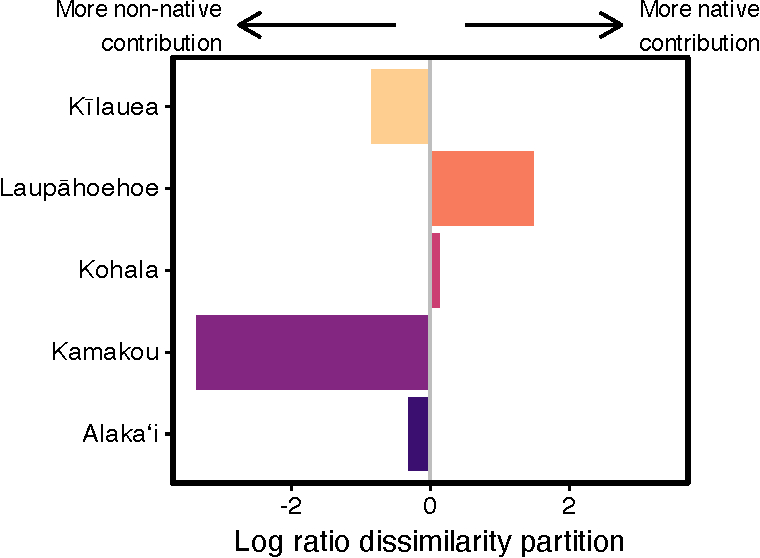
\includegraphics[keepaspectratio]{hawaii-arth-mete-supp_files/figure-pdf/fig-bray-part-1.pdf}}

}

\caption{\label{fig-bray-part}Difference in contribution of native and
non-native species to dissimilarity compared to null. Negative values
indicate greater contribution of non-native species compared to chance
while positive values indicate greater contribution of native species
compared to chance.}

\end{figure}%

\section{Evaluating the consequences of sampling biomass
values}\label{evaluating-the-consequences-of-sampling-biomass-values}

Here we re-run all analyses using a single expected value of biomass
derived from taxon- and stage-specific allometric scaling relationships
rather than sampling with noise from those relationships. To do so we
extract all R code from the qmd file generating this supplement, alter
the metabolic rate estimates going into the METE calculations, and
re-run the code

\begin{Shaded}
\begin{Highlighting}[]
\CommentTok{\# create r script from qmd}
\NormalTok{r\_temp }\OtherTok{\textless{}{-}} \FunctionTok{tempfile}\NormalTok{(}\AttributeTok{fileext =} \StringTok{".R"}\NormalTok{)}
\NormalTok{quarto}\SpecialCharTok{::}\FunctionTok{qmd\_to\_r\_script}\NormalTok{(}\StringTok{"hawaii{-}arth{-}mete{-}supp.qmd"}\NormalTok{, r\_temp)}

\CommentTok{\# remove all chunks subsequent to bray{-}part (including bray{-}part)}
\CommentTok{\# because those do not have to do with IPD}
\NormalTok{r }\OtherTok{\textless{}{-}} \FunctionTok{readLines}\NormalTok{(r\_temp) }
\NormalTok{r }\OtherTok{\textless{}{-}}\NormalTok{ r[}\SpecialCharTok{{-}}\NormalTok{(}\FunctionTok{grep}\NormalTok{(}\StringTok{"label: bray{-}part"}\NormalTok{, r)[}\DecValTok{1}\NormalTok{]}\SpecialCharTok{:}\FunctionTok{length}\NormalTok{(r))]}

\CommentTok{\# remove chunks before \textasciigrave{}mete{-}calc\textasciigrave{}}
\NormalTok{r }\OtherTok{\textless{}{-}}\NormalTok{ r[}\SpecialCharTok{{-}}\NormalTok{(}\DecValTok{1}\SpecialCharTok{:}\NormalTok{(}\FunctionTok{grep}\NormalTok{(}\StringTok{"label: mete{-}calc"}\NormalTok{, r) }\SpecialCharTok{{-}} \DecValTok{1}\NormalTok{))]}

\CommentTok{\# change metabolic rate to expected value}
\NormalTok{r }\OtherTok{\textless{}{-}} \FunctionTok{gsub}\NormalTok{(}\StringTok{"x}\SpecialCharTok{\textbackslash{}\textbackslash{}}\StringTok{$metabolic\_rate"}\NormalTok{,}
          \StringTok{"x}\SpecialCharTok{\textbackslash{}\textbackslash{}}\StringTok{$ind\_biom}\SpecialCharTok{\textbackslash{}\textbackslash{}}\StringTok{\^{}0.75"}\NormalTok{,}
\NormalTok{          r)}

\CommentTok{\# write and source, sourcing into local environment preserves global}
\CommentTok{\# environment}
\FunctionTok{writeLines}\NormalTok{(r, r\_temp)}
\NormalTok{scr\_env }\OtherTok{\textless{}{-}} \FunctionTok{new.env}\NormalTok{()}
\FunctionTok{source}\NormalTok{(r\_temp, }\AttributeTok{local =}\NormalTok{ scr\_env)}
\end{Highlighting}
\end{Shaded}

Now that all analyses involving the IPD have been re-run with expected
values of biomass rather than random draws, we can evaluate differences
between the two approaches.

The first thing to notice is that IPD \(z^2\)-values are correlated
under both analysis scenarios Supplementary Figure~\ref{fig-ipd-both}

\begin{Shaded}
\begin{Highlighting}[]
\FunctionTok{data.frame}\NormalTok{(}\AttributeTok{ipd\_draw =}\NormalTok{ arth\_mete}\SpecialCharTok{$}\NormalTok{z2\_ipd, }
           \AttributeTok{ipd\_expt =}\NormalTok{ scr\_env}\SpecialCharTok{$}\NormalTok{arth\_mete}\SpecialCharTok{$}\NormalTok{z2\_ipd) }\SpecialCharTok{|\textgreater{}} 
    \FunctionTok{ggplot}\NormalTok{(}\FunctionTok{aes}\NormalTok{(ipd\_draw, ipd\_expt)) }\SpecialCharTok{+}
    \FunctionTok{geom\_point}\NormalTok{() }\SpecialCharTok{+}
    \FunctionTok{this\_ms\_look}\NormalTok{(}\AttributeTok{log\_x =} \ConstantTok{TRUE}\NormalTok{, }\AttributeTok{log\_y =} \ConstantTok{TRUE}\NormalTok{) }\SpecialCharTok{+}
    \FunctionTok{geom\_abline}\NormalTok{(}\AttributeTok{intercept =} \DecValTok{0}\NormalTok{, }\AttributeTok{slope =} \DecValTok{1}\NormalTok{) }\SpecialCharTok{+}
    \FunctionTok{xlab}\NormalTok{(}\FunctionTok{expression}\NormalTok{(}\StringTok{"Random draw IPD"}\SpecialCharTok{\textasciitilde{}}\NormalTok{z}\SpecialCharTok{\^{}}\DecValTok{2}\NormalTok{)) }\SpecialCharTok{+}
    \FunctionTok{ylab}\NormalTok{(}\FunctionTok{expression}\NormalTok{(}\StringTok{"Expected value IPD"}\SpecialCharTok{\textasciitilde{}}\NormalTok{z}\SpecialCharTok{\^{}}\DecValTok{2}\NormalTok{))}
\end{Highlighting}
\end{Shaded}

\begin{figure}[H]

\centering{

\pandocbounded{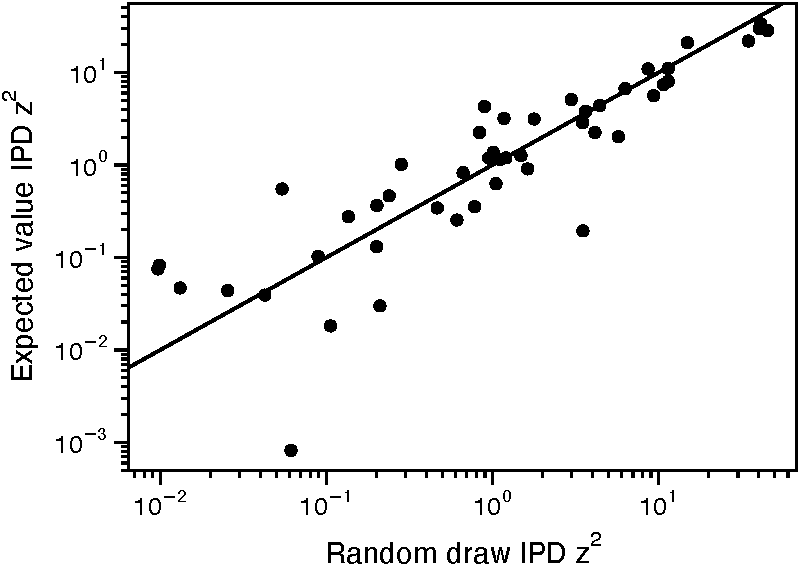
\includegraphics[keepaspectratio]{hawaii-arth-mete-supp_files/figure-pdf/fig-ipd-both-1.pdf}}

}

\caption{\label{fig-ipd-both}Relationship between IPD \(z^2\)-values
when calculated using random draws of expected values of biomass. The
solid line is the 1:1 line.}

\end{figure}%

Using expected values for biomass increases the variability of
log-transformed IPD \(z^2\)-values slightly:
\(SD_\text{expected values}\) = 2.242 compared to
\(SD_\text{random draws}\) = 2.236

This increased variability is not surprising given the artificial
descritization that results from using expected values. We can see the
impact of this descritization by again comparing the exemplar samples
with high and low deviation from Supplementary Figure~\ref{fig-z2-cor}
and Supplementary Figure~\ref{fig-how-diff}. Now we compare on the IPD
\(z^2\) values and see that, while the overall shape of the IPD is
similar, long runs of the same metabolic rate drive both spurious
deviations and conformations to METE predictions Supplementary
Figure~\ref{fig-diff-both}.

\begin{Shaded}
\begin{Highlighting}[]
\FunctionTok{bind\_rows}\NormalTok{(}\AttributeTok{draws =}\NormalTok{ expl\_samps, }
          \AttributeTok{exptd =}\NormalTok{ scr\_env}\SpecialCharTok{$}\NormalTok{expl\_samps, }
          \AttributeTok{.id =} \StringTok{"biomass"}\NormalTok{) }\SpecialCharTok{|\textgreater{}} 
    \FunctionTok{filter}\NormalTok{(dist }\SpecialCharTok{==} \StringTok{"ipd"}\NormalTok{) }\SpecialCharTok{|\textgreater{}} 
    \FunctionTok{ggplot}\NormalTok{(}\FunctionTok{aes}\NormalTok{(rank, m)) }\SpecialCharTok{+}
    \FunctionTok{geom\_point}\NormalTok{(}\FunctionTok{aes}\NormalTok{(rank, abund\_obs)) }\SpecialCharTok{+}
    \FunctionTok{geom\_ribbon}\NormalTok{(}\FunctionTok{aes}\NormalTok{(}\AttributeTok{ymin =}\NormalTok{ lo, }\AttributeTok{ymax =}\NormalTok{ hi), }
                \AttributeTok{fill =} \StringTok{"\#489BC5"}\NormalTok{, }\AttributeTok{alpha =} \FloatTok{0.75}\NormalTok{) }\SpecialCharTok{+}
    \FunctionTok{geom\_line}\NormalTok{(}\AttributeTok{color =} \StringTok{"\#489BC5"}\NormalTok{) }\SpecialCharTok{+}
    \FunctionTok{facet\_grid2}\NormalTok{(}
        \AttributeTok{rows =} \FunctionTok{vars}\NormalTok{(deviation), }\AttributeTok{cols =} \FunctionTok{vars}\NormalTok{(biomass), }
        \AttributeTok{scales =} \StringTok{"free"}\NormalTok{, }\AttributeTok{independent =} \StringTok{"x"}\NormalTok{,}
        \AttributeTok{labeller =} \FunctionTok{as\_labeller}\NormalTok{(}
            \FunctionTok{c}\NormalTok{(}\AttributeTok{hi =} \StringTok{"High deviation"}\NormalTok{, }\AttributeTok{lo =} \StringTok{"Low deviation"}\NormalTok{,}
              \AttributeTok{draws =} \StringTok{"Random draws of biomass"}\NormalTok{, }
              \AttributeTok{exptd =} \StringTok{"Expected values of biomass"}\NormalTok{)}
\NormalTok{        )}
\NormalTok{    ) }\SpecialCharTok{+}
    \FunctionTok{xlab}\NormalTok{(}\StringTok{"Rank"}\NormalTok{) }\SpecialCharTok{+}
    \FunctionTok{ylab}\NormalTok{(}\StringTok{"Metabolic rate"}\NormalTok{) }\SpecialCharTok{+}
    \FunctionTok{this\_ms\_look}\NormalTok{(}\AttributeTok{log\_y =} \ConstantTok{TRUE}\NormalTok{)}
\end{Highlighting}
\end{Shaded}

\begin{figure}[H]

\centering{

\pandocbounded{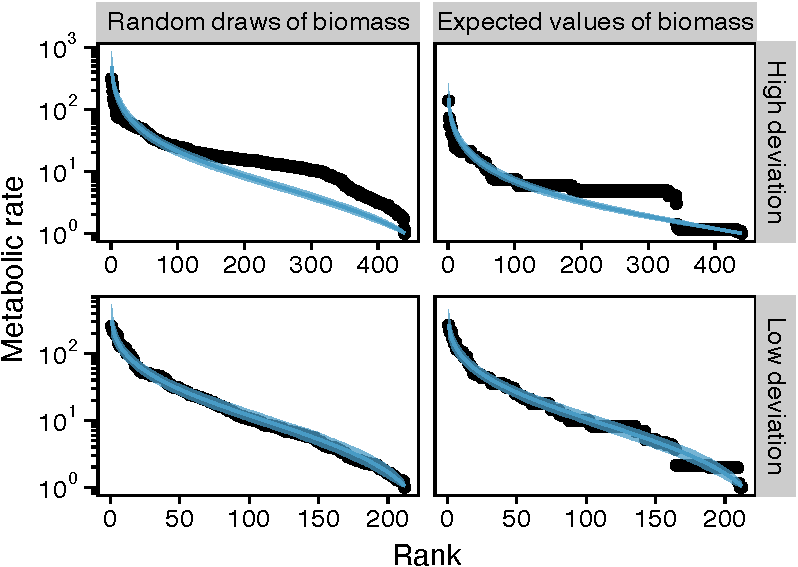
\includegraphics[keepaspectratio]{hawaii-arth-mete-supp_files/figure-pdf/fig-diff-both-1.pdf}}

}

\caption{\label{fig-diff-both}Example rank distributions of individual
metabolic rate showing both high and low deviations from METE as well as
metabolic rate estimates based on random draws from allometric
relationships versus the expected values of those relationships. Note
that with expected values artificial descritization causes both spurious
deviation from METE (as in the low deviation example) and spurios
conformations to METE (as in the high deviation example).}

\end{figure}%

The primary effect of increased variability in IPD \(z^2\)-values and
spurious deviations/conformations is to decrease the significance of the
relationship of IPD \(z^2\)-values and explanatory variables. While LRT
identified both proportion non-native species and dissimilarity as
predictors of IPD \(z^2\)-values, when using expected values of biomass
the \(P\)-values of these relationships are no longer \(\leq 0.05\):

\begin{Shaded}
\begin{Highlighting}[]
\CommentTok{\# LRT of proportion non{-}native species}
\FunctionTok{anova}\NormalTok{(scr\_env}\SpecialCharTok{$}\NormalTok{ipd\_rma\_non)}
\end{Highlighting}
\end{Shaded}

\begin{verbatim}

Test of Moderators (coefficient 2):
QM(df = 1) = 2.8824, p-val = 0.0895
\end{verbatim}

\begin{Shaded}
\begin{Highlighting}[]
\CommentTok{\# LRT of dissimilarity}
\FunctionTok{anova}\NormalTok{(scr\_env}\SpecialCharTok{$}\NormalTok{ipd\_rma\_diss)}
\end{Highlighting}
\end{Shaded}

\begin{verbatim}

Test of Moderators (coefficient 2):
QM(df = 1) = 2.5978, p-val = 0.1070
\end{verbatim}

It should be noted, however, that there is still marginal support for
these relationships based on 95\% confidence intervals of their
coefficients in the two models:

\begin{Shaded}
\begin{Highlighting}[]
\CommentTok{\# slope of proportion non{-}native species}
\FunctionTok{confint}\NormalTok{(scr\_env}\SpecialCharTok{$}\NormalTok{ipd\_rma\_non, }\AttributeTok{fixed =} \ConstantTok{TRUE}\NormalTok{, }\AttributeTok{random =} \ConstantTok{FALSE}\NormalTok{) }\SpecialCharTok{|\textgreater{}} 
    \FunctionTok{as.data.frame}\NormalTok{() }\SpecialCharTok{|\textgreater{}} 
\NormalTok{    (\textbackslash{}(x) x[}\DecValTok{2}\NormalTok{, , }\AttributeTok{drop =} \ConstantTok{FALSE}\NormalTok{])()}
\end{Highlighting}
\end{Shaded}

\begin{verbatim}
                  estimate     ci.lb    ci.ub
prop_nspp_non_nat  16.7525 -2.587085 36.09208
\end{verbatim}

\begin{Shaded}
\begin{Highlighting}[]
\CommentTok{\# slope of dissimilarity}
\FunctionTok{confint}\NormalTok{(scr\_env}\SpecialCharTok{$}\NormalTok{ipd\_rma\_diss, }\AttributeTok{fixed =} \ConstantTok{TRUE}\NormalTok{, }\AttributeTok{random =} \ConstantTok{FALSE}\NormalTok{) }\SpecialCharTok{|\textgreater{}} 
    \FunctionTok{as.data.frame}\NormalTok{() }\SpecialCharTok{|\textgreater{}} 
\NormalTok{    (\textbackslash{}(x) x[}\DecValTok{2}\NormalTok{, , }\AttributeTok{drop =} \ConstantTok{FALSE}\NormalTok{])()}
\end{Highlighting}
\end{Shaded}

\begin{verbatim}
           estimate       ci.lb     ci.ub
mean_diss 0.1414801 -0.03056349 0.3135237
\end{verbatim}

In both cases, the 95\% CIs contain a majority of positive values.

\phantomsection\label{refs}
\begin{CSLReferences}{1}{0}
\bibitem[\citeproctext]{ref-quarto}
Allaire, J.J., Teague, C., Scheidegger, C., Xie, Y., Dervieux, C. \&
Woodhull, G. (2025).
\href{https://doi.org/10.5281/zenodo.5960048}{{Quarto}}.

\end{CSLReferences}




\end{document}
